\chapter{工程机器人与高级构型}
\label{ch:engineer}

\begin{introduction}
  \item 看懂工程项目的模式、动作行与“每 20\,ms 从上到下执行一次”的程序模型；
  \item 学会关闭预制四轮底盘，把释放出来的引脚重新分配给电机和舵机；
  \item 理解麦克纳姆轮、全向轮、舵轮和机械臂逆解的结构与运动学；
  \item 用“变量 + 受限表达式”写出四轮麦轮混控和二自由度机械臂逆解；
  \item 用试算、表达式编译检查、生成代码和实机低速测试完成校准与排错。
\end{introduction}

本章讨论的“高级构型”，指的是预制四轮差速底盘之外的移动机构与执行机构：
麦克纳姆轮、全向轮、舵轮，以及由舵机驱动的机械臂。它们在 RoboMaster
赛场上并不罕见，但对控制的要求比“左摇杆前后、右摇杆转向”高得多。
PIE-Block 的工程项目提供了两样关键能力：一是可以把预制底盘整体关掉，
自己分配每一个输出；二是可以用变量和受限表达式描述多输入、多输出的
控制律。本章就围绕这两样能力展开。

图~\ref{fig:ch05-photo-rm} 是一台真实的 RoboMaster 机器人：独立悬挂的
底盘、顶部的云台与发射机构，都是赛场上经过验证的工程构型。本章的任务，
是用 PIE-Block 把这类构型中适合开环控制的部分——麦轮、全向轮和舵机
机械臂——配置出来。

\begin{figure}[htbp]
  \centering
  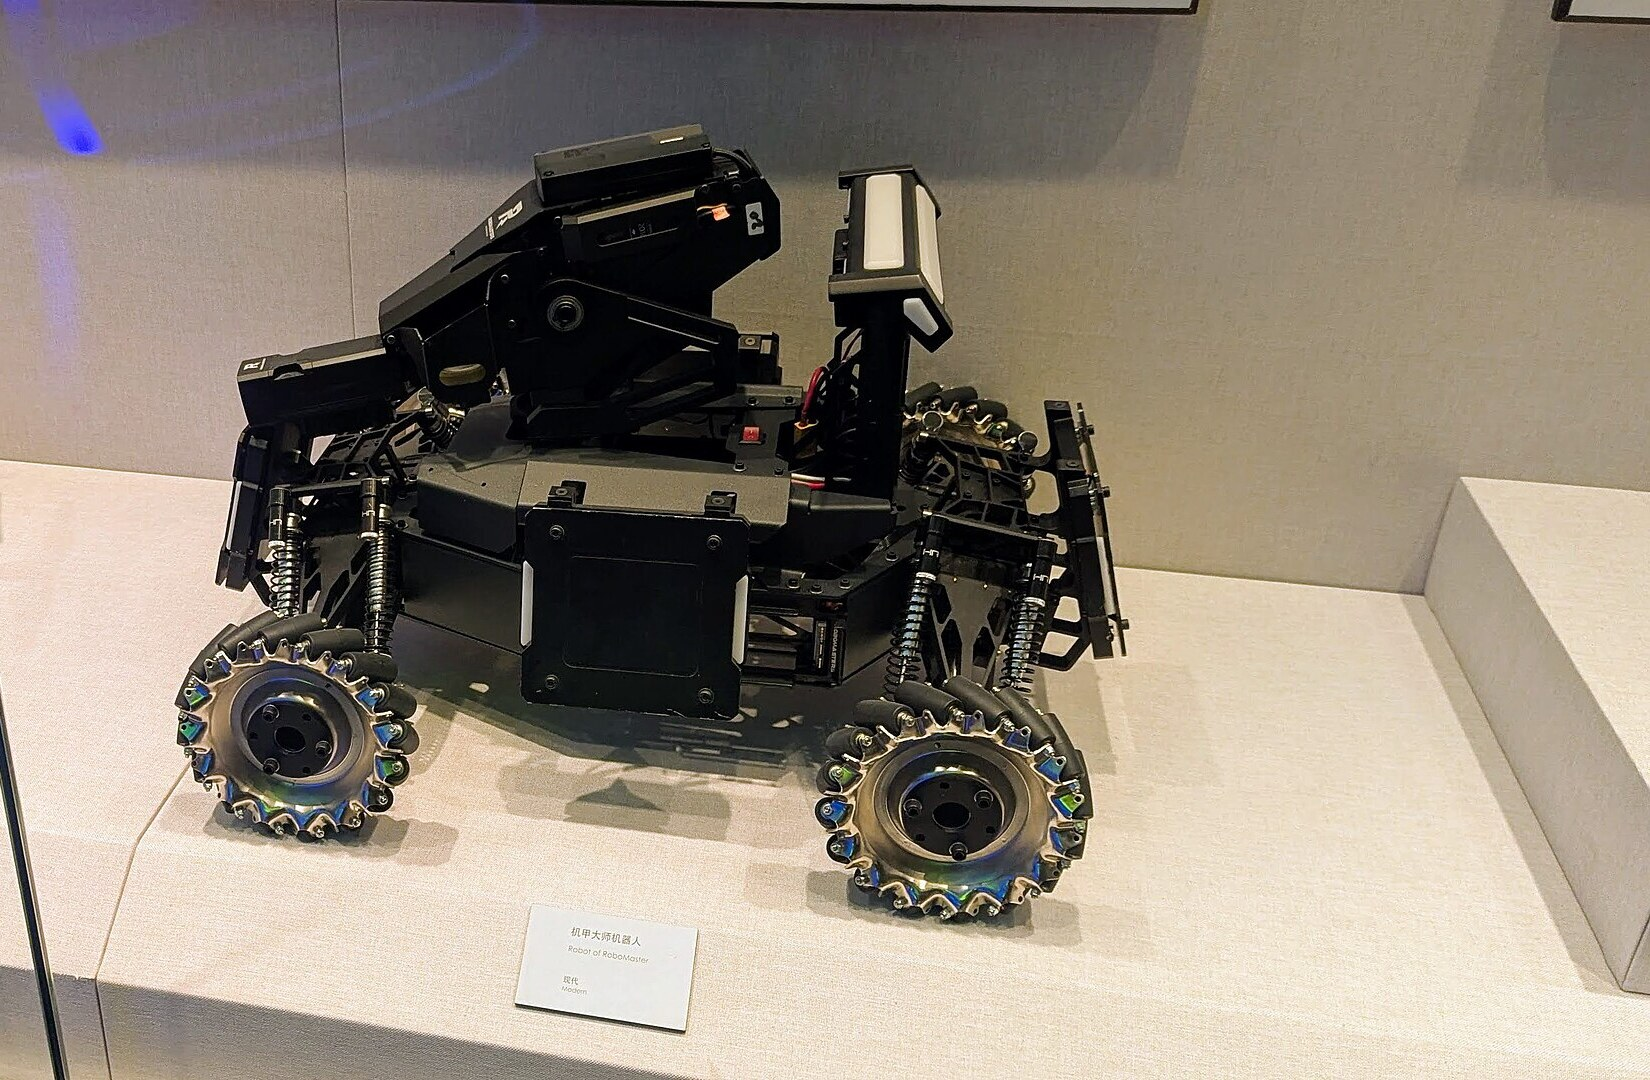
\includegraphics[width=0.82\linewidth]{image/ch05/photo-robomaster.jpg}
  \caption{RoboMaster 机器人展品（深圳南山博物馆）：底盘带独立悬挂，顶部
  是云台与发射机构（照片：Underbar dk，Wikimedia Commons，CC BY-SA 4.0）}
  \label{fig:ch05-photo-rm}
\end{figure}

需要先说明本章的边界。PIE-Block 不是任意 C 语言编程环境：表达式只能是
一条右值表达式，没有语句、循环和自定义函数；生成代码只读，改配置才会
重新生成；所有控制都是开环的，扩展板没有编码器回读。因此本章的示例
都限定在“闭式运动学 + 开环输出”的范围内。舵轮和 4 自由度及以上机械臂（以及 3 自由度的世界坐标目标）的
完整实现超出了当前工具的能力，本章会明确说明边界，不把“理论上可以拼”
写成“开箱即用”。

\section{工程项目的“程序”}

\subsection{模式、动作行与执行顺序}

工程项目最多有 4 个模式。每个模式是一张独立的动作表，固件每轮主循环
只执行当前模式对应的函数 \texttt{RunMode1()}、\texttt{RunMode2()} 等。
动作表按列表顺序从上到下执行，执行频率约为 50\,Hz（主循环一轮约
20\,ms）。这张表就是本章所说的“程序”。

动作行的字段组合决定它的语义，共四种：

\begin{enumerate}
  \item \textbf{遥控输入 → 引脚}：传统动作，如按键控制舵机、摇杆控制电机。
        方向、控制方式和参数按固定控制律生效。
  \item \textbf{未指定 → 引脚}：计算行。每轮把一条表达式的值直接写到引脚，
        不经过方向、控制方式和参数。
  \item \textbf{遥控输入 → 整数/有理数}：把输入值赋给变量。
  \item \textbf{未指定 → 整数/有理数}：每轮把表达式的值赋给变量。
\end{enumerate}

只有“输入”选为“未指定”的行才能填写表达式。表达式允许字面量、变量、
内置输入 \texttt{LX/LY/RX/RY}、按键别名、四则运算、取模、括号、比较、
逻辑、三元运算，以及 \texttt{abs/min/max/sign/sqrt/atan2} 和常量
\texttt{PI/E}；不允许分号、花括号、赋值、下标和逗号运算符。换句话说，它是一条
可以嵌套函数调用的右值表达式，而不是一小段 C 代码。

变量有两个作用域。只在一个模式里出现的变量是该模式的局部变量，必须在
同一模式内先定义后使用，生成代码时声明在 \texttt{RunModeN()} 开头；
同名变量出现在两个及以上模式时提升为全局变量，类型必须一致，未赋值的
周期保持上一次的值。局部变量适合做中间量，例如逆解里的 \texttt{c2}；
全局变量适合跨模式共享常量或状态，但要清楚它每一轮都可能被重新赋值。

\begin{note}
列表顺序就是执行顺序。拖动动作行左侧的手柄即可调整顺序；变量行必须排在
引用它的行之前。
\end{note}

模式切换时，固件调用 \texttt{PrepareMode()}：新模式下没有被动作行映射的
电机和抖动电机清零，舵机保持最后位置；摩擦轮走专用安全栈，\texttt{PrepareMode}
不会把它归零，状态跨模式保持。
工程项目关闭预制底盘后，不再有“保留左摇杆底盘控制”这个选项；每个模式
必须自己把需要运动的轮子写全。这一点在后面的麦轮示例里会反复用到。

\subsection{关闭预制底盘：释放四路电机}

工程项目默认启用预制四轮差速底盘。启用时，四个轮子的引脚、方向和普通
速度都是必填项，生成代码会调用 \texttt{CalculateChassis()} 做左摇杆差速
混控。对麦轮、全向轮这类需要自定义混控的底盘，这个预制层反而碍事。

在“遥控器与底盘”页关闭“启用底盘控制”后：

\begin{itemize}
  \item 四个底盘引脚被释放，可以在“PWM 与引脚”里重新指定角色；
  \item “普通速度”“冲刺速度”“转向反转”等底盘参数不再必填；
  \item 模式 1 的“保留左摇杆底盘控制”开关消失，模式里不能再设置
        \texttt{preserveChassis}；
  \item 生成的代码不再包含 \texttt{CalculateChassis()}，四路输出完全由
        动作行决定。
\end{itemize}

关闭开关后，页面会提示“未启用预制四轮底盘：原底盘引脚已释放给动作行
使用”，如图~\ref{fig:ch05-chassis-off} 所示。注意这只是“释放”，并不会
自动把四个轮子变成电机：还需要到“PWM 与引脚”页给每个脚指定角色和
PWM 组频率。

\begin{figure}[htbp]
  \centering
  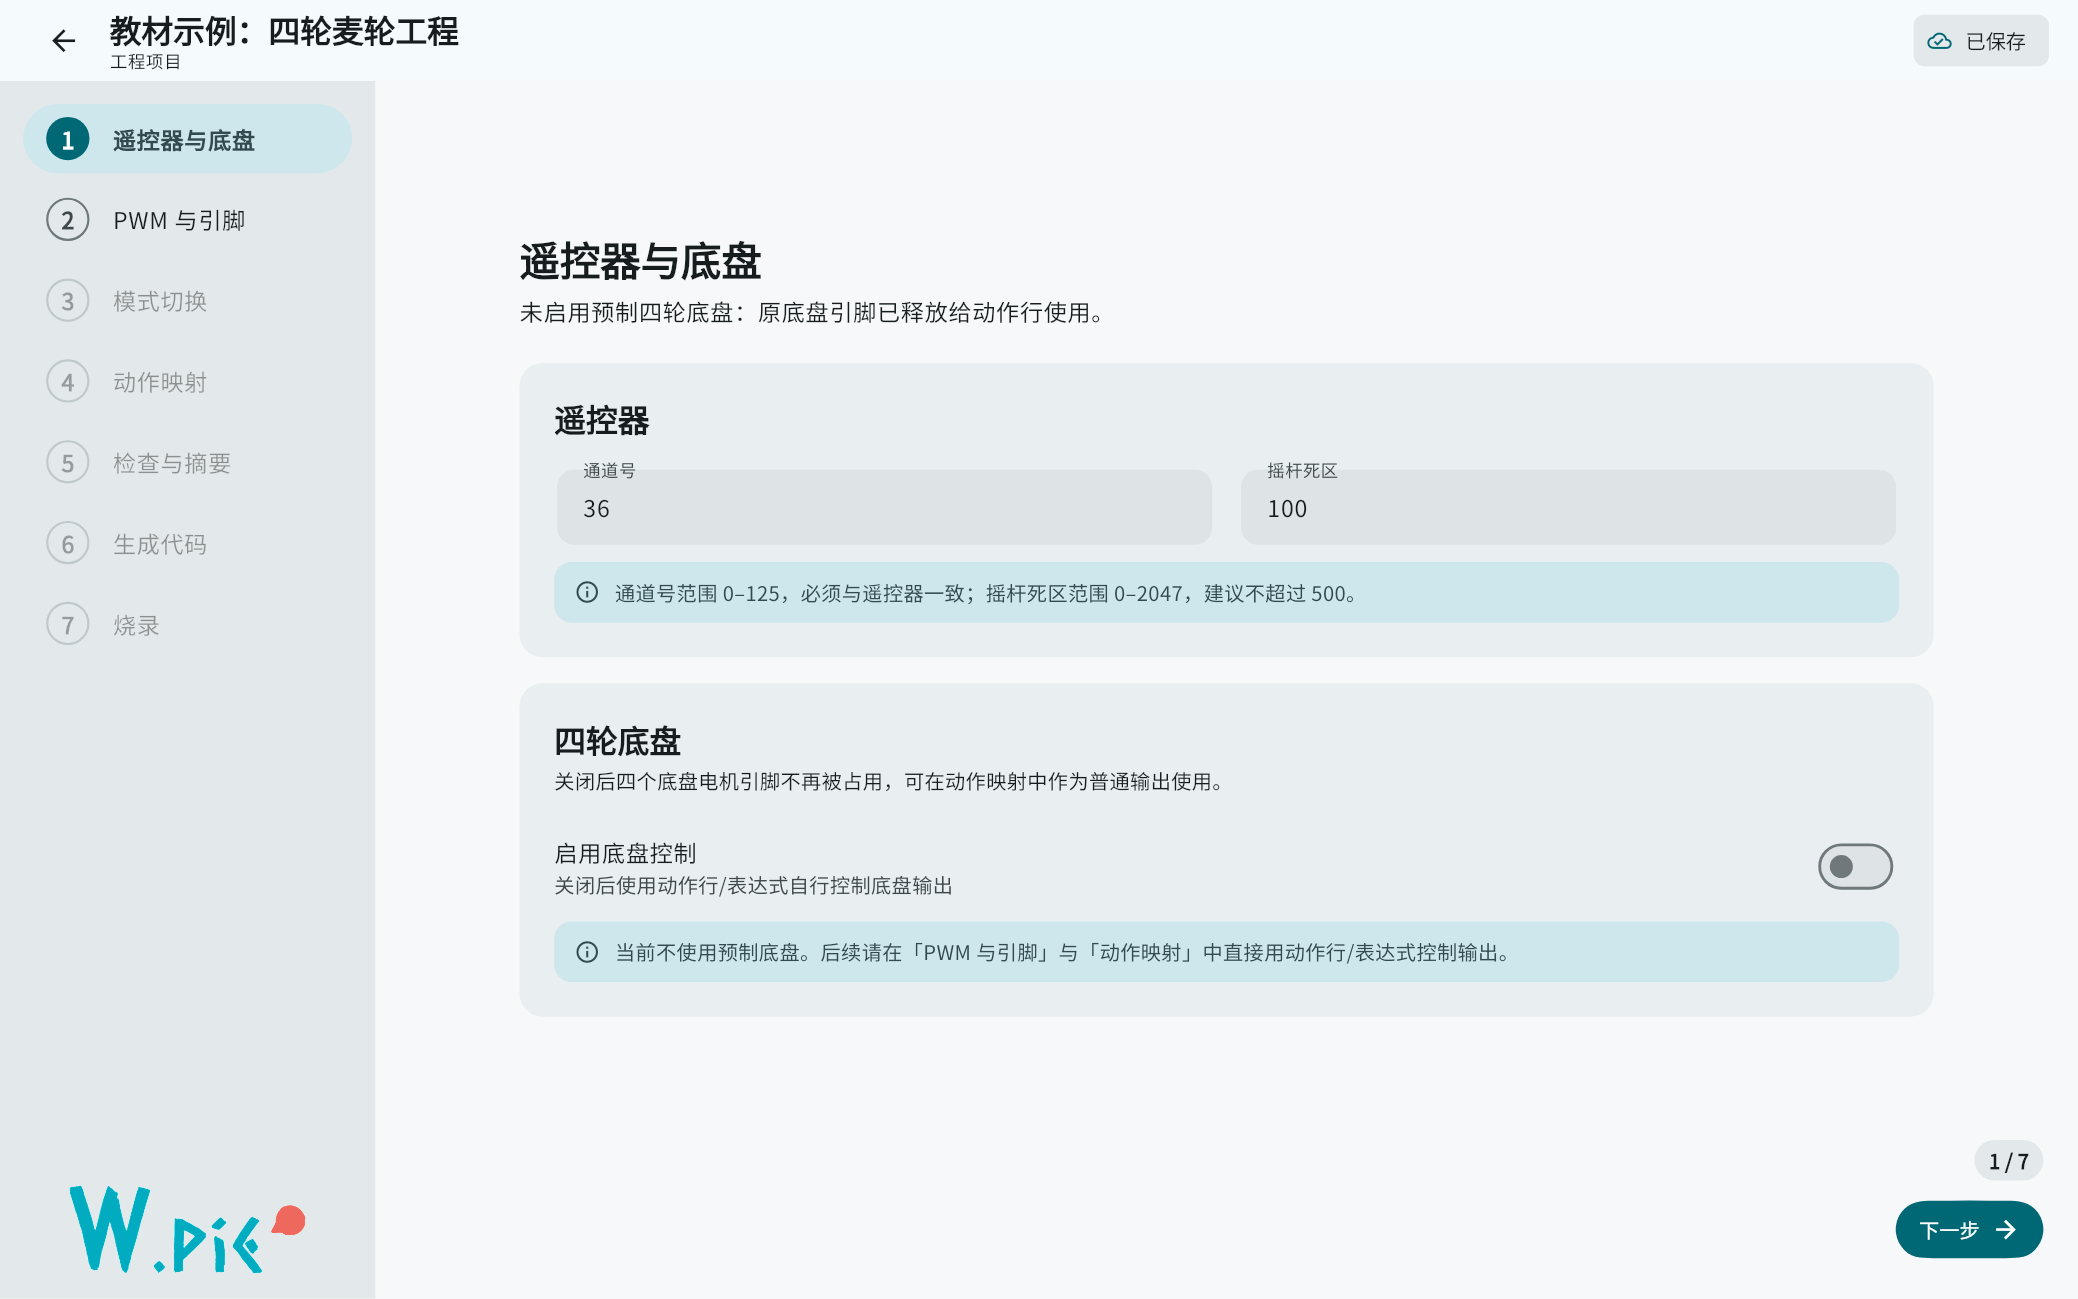
\includegraphics[width=0.94\linewidth]{image/ch05/5-1-chassis-off.png}
  \caption{关闭“启用底盘控制”后的“遥控器与底盘”页。四个底盘脚被释放，
  页面提示后续用动作行/表达式控制输出}
  \label{fig:ch05-chassis-off}
\end{figure}

\subsection{输出单位、坐标系与资源账本}

工程项目的 8 路扩展输出分成两组，组内共享频率：

\begin{center}
\begin{tabular}{@{}lll@{}}
\toprule
PWM 组 & 引脚 & 常用频率 \\
\midrule
PWMA & P60、P62、P64、P66 & 50\,Hz（舵机/摩擦轮）或 10000\,Hz（电机） \\
PWMB & P74、P75、P76、P77 & 50\,Hz（舵机/摩擦轮）或 10000\,Hz（电机） \\
\bottomrule
\end{tabular}
\end{center}

其中 P60、P62、P74、P75、P76、P77 可以作电机；P64、P66 可以作摩擦轮
或舵机；8 个扩展脚都可以作舵机；主控板另有 MP03、MP74 两个固定 50\,Hz
的主舵机口。P64、P66 虽然可以改成舵机，但不能同时当摩擦轮用。
P60、P62、P74--P77 还可以设为“抖动电机”，用于小幅度抖动；抖动电机
工作在 50\,Hz，不是连续驱动，本章示例不涉及。

\begin{remark}
默认四轮底盘用的正是 PWMB 的 P74--P77。因此把四轮改成麦轮时，最自然的
分配是：四个轮子继续用 P74--P77，PWMB 设 10000\,Hz；PWMA 设 50\,Hz，
留给机械臂舵机。这样既沿用了原来的接线习惯，又给舵机留出了一整组
50\,Hz 输出。如果反过来把轮子分到 PWMA 和 PWMB 两组，两组都必须
10000\,Hz，扩展舵机就没有 50\,Hz 的落脚点了。
\end{remark}

输出单位按引脚角色决定。电机是最多 $\pm10000$ 的 duty；舵机是
$-90^\circ$ 到 $+90^\circ$ 的角度，生成代码时自动换算成 250--1250 的
绝对占空比；变量按声明类型保存，整数用 \texttt{int32\_t}，有理数用
\texttt{float}。表达式行写电机的 duty 真值，写舵机的角度真值，写变量的
声明类型值；生成器负责钳位和类型转换。

本章反复出现的术语先集中列在表~\ref{tab:ch05-terms} 里，后面各节会给出
结构图和公式。

\begin{table}[htbp]
  \centering
  \small
  \begin{tabularx}{\linewidth}{@{}l l >{\raggedright\arraybackslash}X@{}}
    \toprule
    术语 & 英文 & 一句话解释 \\
    \midrule
    麦克纳姆轮 & Mecanum wheel & 轮毂斜装 $45^\circ$ 辊子的全向轮；四轮斜向力可合成平移和自转 \\
    全向轮 & Omni wheel & 轮缘装 $90^\circ$ 辊子的轮子；只能沿滚动方向出力，侧向自由滑动 \\
    舵轮 & Swerve module & 可绕竖直轴转向的驱动轮模块；每个模块有转向和驱动两个执行器 \\
    正运动学 & Forward kinematics & 已知关节角，求末端位置 \\
    逆运动学 & Inverse kinematics & 已知末端目标，求关节角；本章只做闭式解 \\
    工作空间 & Workspace & 末端能够到达的位置集合；二连杆是一个圆环 \\
    混控 & Mixing & 把车体平移/自转指令分配到多个执行器的过程 \\
    占空比 & Duty & PWM 高电平比例；本项目电机用 $\pm10000$，舵机用 250--1250 \\
    \bottomrule
  \end{tabularx}
  \caption{本章术语速查}
  \label{tab:ch05-terms}
\end{table}

本章统一约定：机体坐标系 $x$ 轴向前、$y$ 轴向左，偏航逆时针为正；
手柄推上时 \texttt{LY} 为负、推右时 \texttt{LX} 为正。示例用
\texttt{vx = -LY}、\texttt{vy = -LX} 换算成“前为正、左为正”的速度。
不同批次手柄的标定可能相反，第一次上车时务必用试算和低速点动核对四个
方向；如果反了，把这两个变量的符号改掉即可。

\section{麦克纳姆轮}

\subsection{45$^\circ$ 辊子与斜向推力}

麦克纳姆轮（Mecanum wheel，常简称“麦轮”，也见“迈克纳姆轮”的写法）的
轮毂周围斜装着许多小辊子，
辊子轴线与轮子平面成 $45^\circ$。轮子转动时，辊子与地面接触点产生的力
不再只沿轮子前进方向，而是分解成两个分量：一个沿轮子前进方向，另一个
沿垂直于轮子的方向。四个轮子按对角线成对安装，让这些斜向分量在需要时
叠加、在不需要时抵消，就能合成前后、左右甚至自转的运动。

图~\ref{fig:ch05-mecanum} 左侧是四轮俯视布局：四个轮子分别位于左前、
左后、右前、右后，轮子长边沿前后方向；右侧是单个轮子的受力分解。实际
装配时左右两侧轮子的辊子方向是镜像的，接线或表达式里用符号修正即可。

\begin{figure}[htbp]
  \centering
  \begin{minipage}{0.58\linewidth}
    \centering
    \begin{tikzpicture}[scale=0.78,>=Latex,font=\small,
      body/.style={draw=structurecolor!70,fill=structurecolor!6,
        rounded corners=3pt,line width=0.9pt},
      wheel/.style={draw=black!65,fill=gray!12,
        rounded corners=1.5pt,line width=0.7pt},
      roller/.style={draw=black!45,line width=0.45pt},
      axis/.style={-{Latex[length=2.2mm]},line width=1.1pt,structurecolor},
      lab/.style={font=\small,inner sep=1pt}]
      % 车体：左右为 y，前后为 x
      \draw[body] (-2.6,-3.0) rectangle (2.6,3.0);
      % 四个轮子：在车体四角，长边沿前后方向
      % 麦轮左右两侧的辊子方向镜像：左前/右后同向，右前/左后同向。
      \foreach \x/\y/\s in {-2.25/1.9/1, 2.25/-1.9/1,
                            2.25/1.9/-1, -2.25/-1.9/-1} {
        \draw[wheel] (\x-0.28,\y-1.05) rectangle (\x+0.28,\y+1.05);
        \foreach \t in {-0.85,-0.45,-0.05,0.35,0.75} {
          \draw[roller]
            (\x-0.28,\y+\t-0.28*\s) -- (\x+0.28,\y+\t+0.28*\s);
        }
      }
      % 车轮中心与标签
      \node[lab] at (-2.25,3.25) {左前};
      \node[lab] at (2.25,3.25) {右前};
      \node[lab] at (-2.25,-3.25) {左后};
      \node[lab] at (2.25,-3.25) {右后};
      % 坐标系
      \draw[axis] (0,0) -- (0,3.9) node[above] {$x$ 向前};
      \draw[axis] (0,0) -- (-3.9,0) node[left] {$y$ 向左};
      \node[lab,below] at (0,-0.25) {俯视};
    \end{tikzpicture}
  \end{minipage}\hfill
  \begin{minipage}{0.38\linewidth}
    \centering
    \begin{tikzpicture}[scale=0.82,>=Latex,font=\small,
      wheel/.style={draw=black!65,fill=gray!12,
        rounded corners=2pt,line width=0.8pt},
      roller/.style={draw=black!45,line width=0.5pt},
      force/.style={-{Latex[length=2mm]},line width=1pt,second},
      axis/.style={-{Latex[length=2mm]},line width=0.8pt,structurecolor},
      lab/.style={font=\small,inner sep=1pt}]
      \draw[wheel] (-0.9,-2.1) rectangle (0.9,2.1);
      \foreach \t in {-1.75,-1.15,-0.55,0.05,0.65,1.25} {
        \draw[roller] (-0.45,\t-0.45) -- (0.45,\t+0.45);
      }
      \draw[axis] (0,-2.4) -- (0,3.0) node[above] {$v$};
      % 分量记号与本章坐标系一致：x 沿滚动方向（前进），y 为侧向
      \draw[force] (0,0) -- (0.9,0.9) node[right] {$F$};
      \draw[force,dashed] (0,0) -- (0,0.9) node[left] {$F_x$};
      \draw[force,dashed] (0,0) -- (0.9,0) node[below right] {$F_y$};
      \node[lab] at (0.25,-2.7) {辊子 $45^\circ$};
    \end{tikzpicture}
  \end{minipage}
  \caption{麦克纳姆轮：四轮俯视布局（左）与单轮斜向力的分解（右）}
  \label{fig:ch05-mecanum}
\end{figure}

真实的麦克纳姆轮如图~\ref{fig:ch05-photo-mecanum} 所示：辊子斜装在轮毂
四周，与轮面约成 $45^\circ$；成对购买时分为左旋与右旋两种，装配时左右
两侧镜像。

\begin{figure}[htbp]
  \centering
  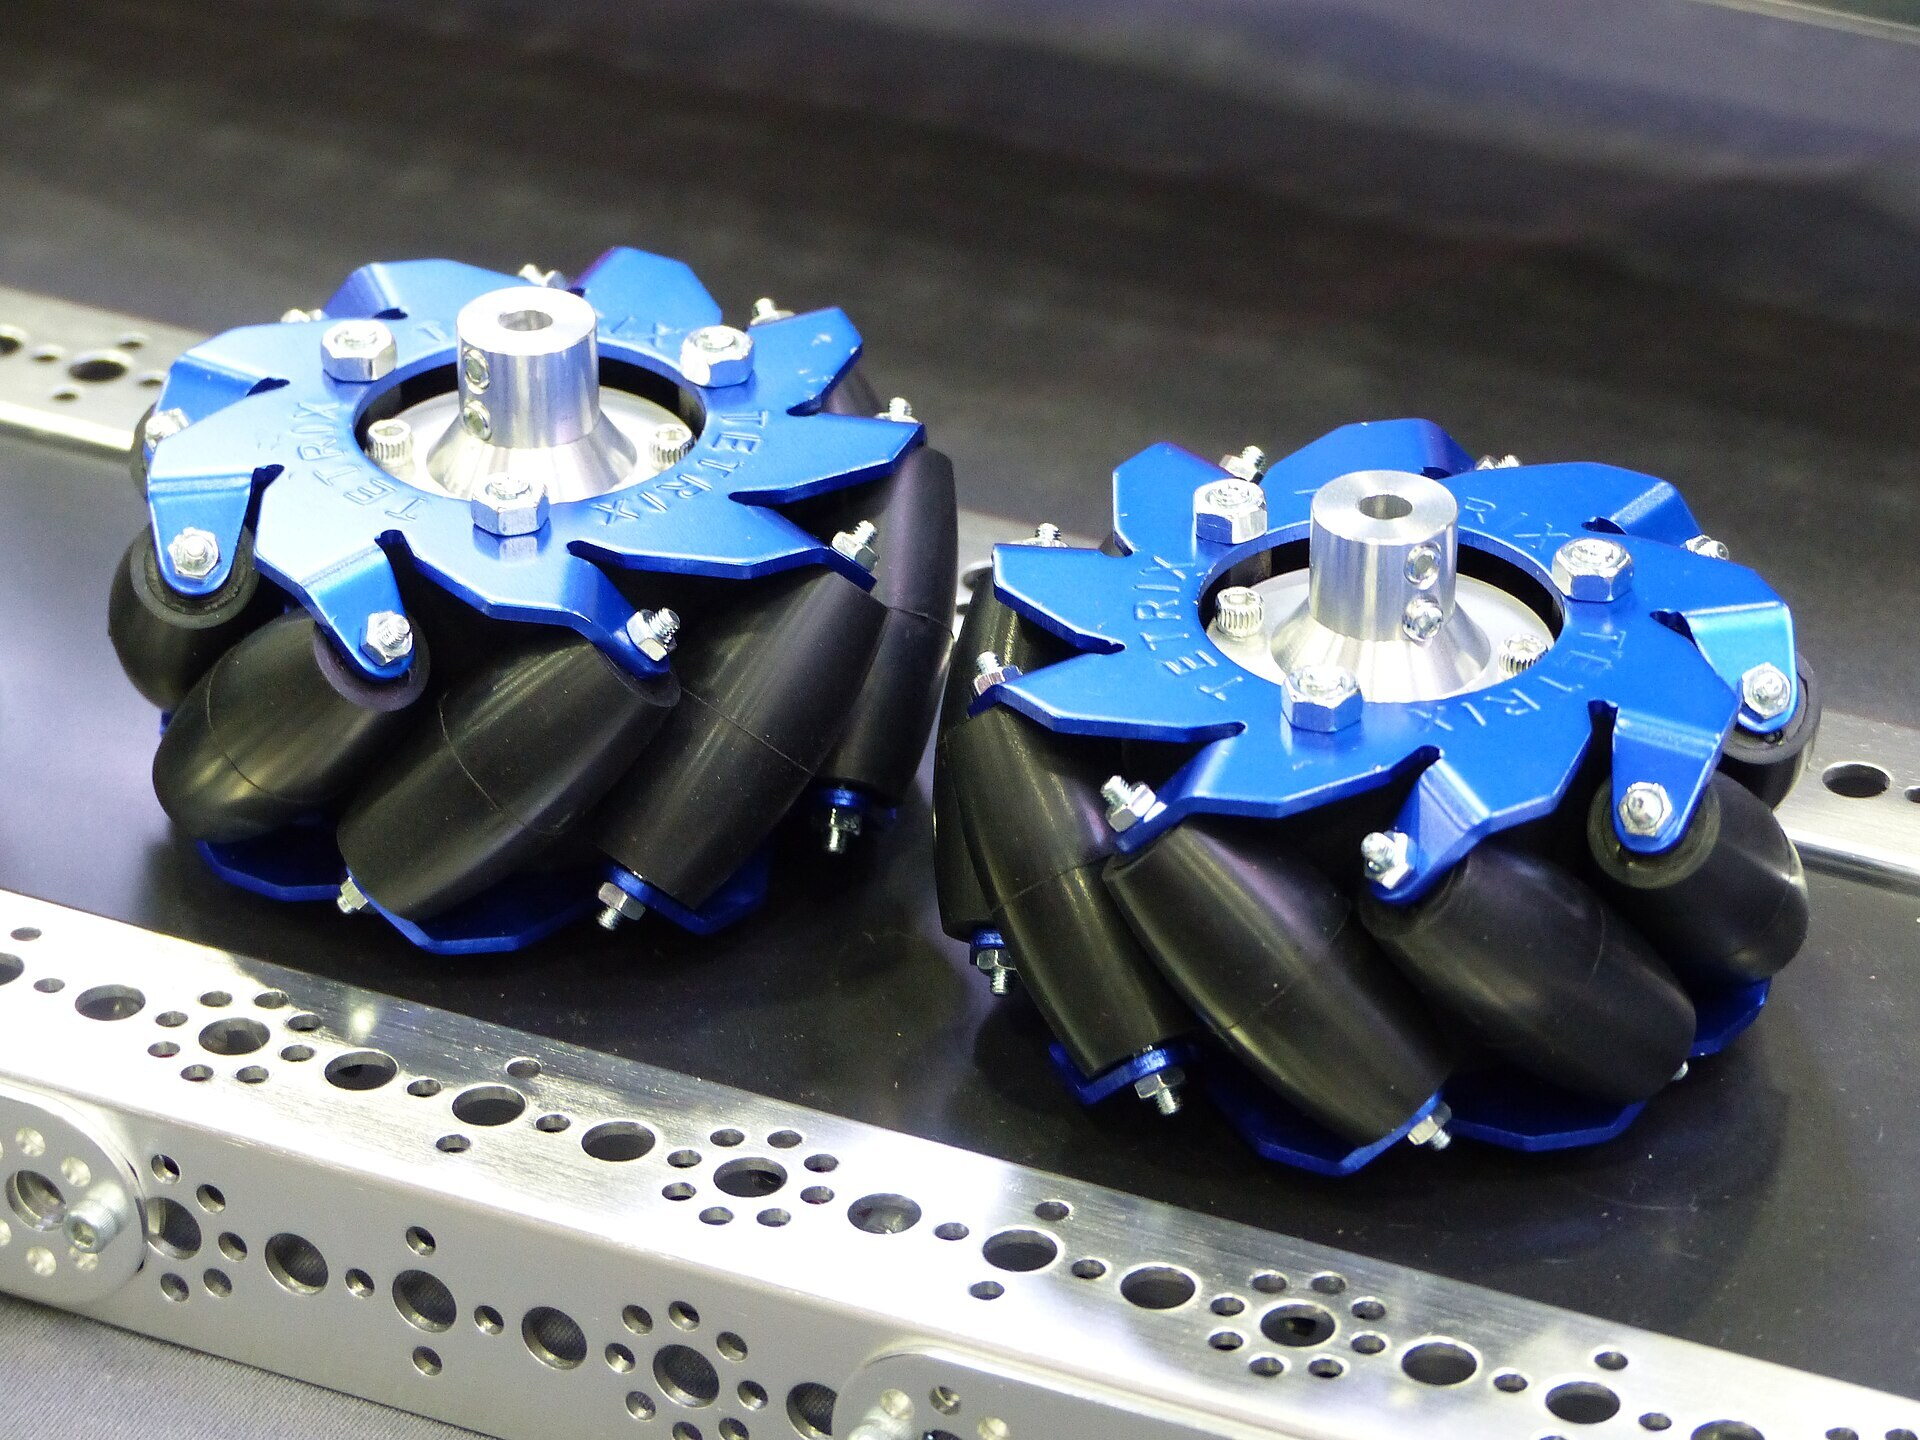
\includegraphics[width=0.78\linewidth]{image/ch05/photo-mecanum.jpg}
  \caption{真实的麦克纳姆轮：轮毂周围斜装着约 $45^\circ$ 的辊子
  （照片：Stilfehler，Wikimedia Commons，CC BY-SA 4.0）}
  \label{fig:ch05-photo-mecanum}
\end{figure}

\subsection{四轮平移运动学}

先只考虑前后和左右平移，不考虑自转。设四个轮子沿前进方向的线速度为
$v_{\mathrm{FL}}$、$v_{\mathrm{FR}}$、$v_{\mathrm{RL}}$、$v_{\mathrm{RR}}$，
车体速度为 $v_x$（前）和 $v_y$（左），在理想辊子、无打滑、四轮对称的
假设下：

\begin{equation}
\begin{aligned}
v_{\mathrm{FL}} &= v_x - v_y, &
v_{\mathrm{FR}} &= v_x + v_y, \\
v_{\mathrm{RL}} &= v_x + v_y, &
v_{\mathrm{RR}} &= v_x - v_y.
\end{aligned}
\label{eq:ch05-mecanum}
\end{equation}

直观解释：纯前进时四个轮子同速；纯左移时左前和右后反转、右前和左后正转；
斜向运动时四个轮子按两个方向的组合分配速度。每个轮子的线速度再按
满量程归一化，就能得到电机 duty：

\begin{equation}
d_i = \operatorname{clamp}\left(\frac{v_i}{2047}\cdot 10000,\,-10000,\,10000\right).
\label{eq:ch05-duty}
\end{equation}

由于摇杆 $v_x$、$v_y$ 各自的范围是 $\pm2047$，$v_x\pm v_y$ 可能达到
$\pm4094$。采用上式时，纯前进和纯横移都能到满速，但对角线方向会有一对
轮子算出 $\pm20000$，被钳位到 $\pm10000$。这保证了方向不反，但速度不再
严格线性。更好的做法是每轮根据四个轮子的最大值做动态归一化，但那需要
额外的比较和除法；本工具支持在表达式里写 \texttt{min/max/abs}，但示例
优先选择简单、可解释的固定缩放，并在“边界”一节说明代价。

如果不需要自转，式~\eqref{eq:ch05-mecanum} 就是完整的混控。需要自转时，
给四个轮子加上偏航项（$\omega$ 为偏航角速度，$L$、$W$ 为轴距和轮距）：

\begin{equation}
\begin{aligned}
v_{\mathrm{FL}} &= v_x - v_y - \tfrac{L+W}{2}\omega, &
v_{\mathrm{FR}} &= v_x + v_y + \tfrac{L+W}{2}\omega, \\
v_{\mathrm{RL}} &= v_x + v_y - \tfrac{L+W}{2}\omega, &
v_{\mathrm{RR}} &= v_x - v_y + \tfrac{L+W}{2}\omega.
\end{aligned}
\label{eq:ch05-mecanum-yaw}
\end{equation}

式~\eqref{eq:ch05-mecanum-yaw} 需要一路偏航输入。智能手柄没有陀螺仪，
只能用右摇杆 \texttt{RX} 做开环自转；本示例把 \texttt{RX} 留给机械臂，
因此主示例不做自转，只在“修改与校准”里给出加入方法。

\subsection{示例 A：四轮麦轮工程车}

\paragraph*{硬件假设}
四个麦轮分别接 P74（左前）、P75（左后）、P76（右前）、P77（右后），
每个轮子一个驱动电机；PWMB 设 10000\,Hz。PWMA 设 50\,Hz，本示例暂不接
扩展舵机，P60/P62/P64/P66 都设为“未使用”。机械臂示例会单独使用主舵机
MP03/MP74；把两个示例合并时，PWMA 的 50\,Hz 正好可以留给机械臂。

\paragraph*{配置步骤}
\begin{enumerate}
  \item 新建“工程项目”，填写项目名称；在“遥控器与底盘”页填写通道号
        36、死区 100，关闭“启用底盘控制”。
  \item 进入“PWM 与引脚”：PWMA 选 50\,Hz，PWMB 选 10000\,Hz；
        P74、P75、P76、P77 的角色选“平滑电机”，P60、P62、P64、P66
        选“未使用”。如图~\ref{fig:ch05-pwm-pins} 所示。
  \item 进入“模式切换”，模式数量选 1。模式数大于 1 时才需要填写切换
        策略和切换按键；本示例不需要。
  \item 进入“动作映射”，按表~\ref{tab:ch05-mecanum-rows} 添加 6 行。
        每行先选“输入 = 未指定”，再选输出：变量行选“整数”，引脚行选
        P74--P77；变量行填写变量名，所有行填写表达式。
\end{enumerate}

\begin{figure}[htbp]
  \centering
  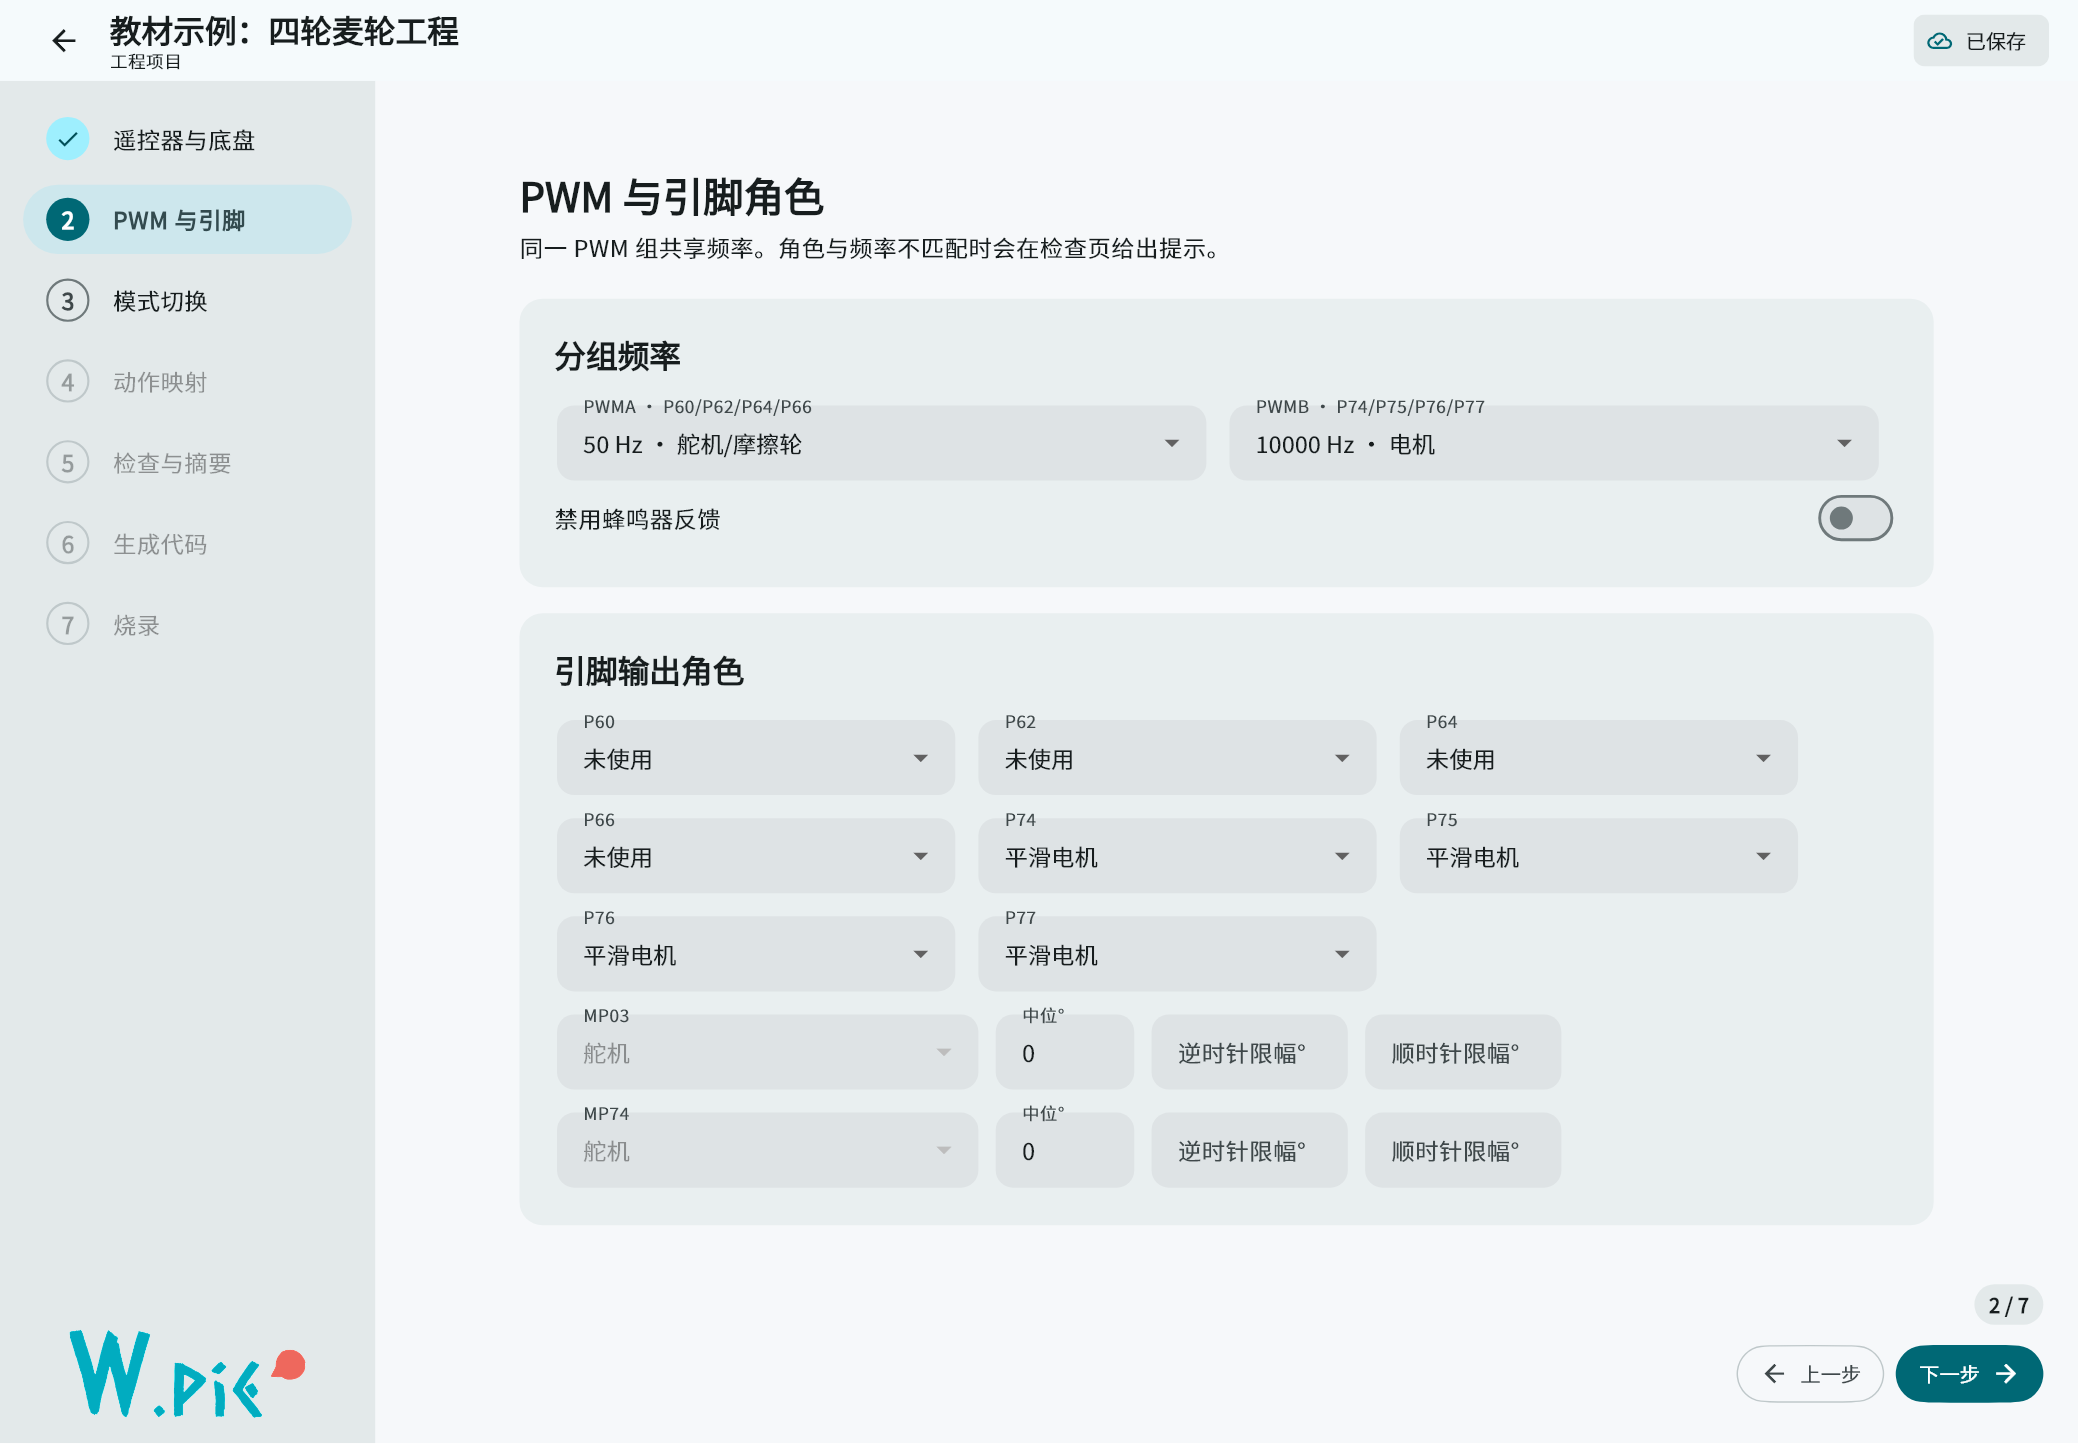
\includegraphics[width=0.90\linewidth]{image/ch05/5-2-pwm-pins.png}
  \caption{示例 A 的“PWM 与引脚”页：PWMB 为 10000\,Hz，P74--P77 为平滑电机；
  PWMA 留 50\,Hz 给后续舵机}
  \label{fig:ch05-pwm-pins}
\end{figure}

\begin{table}[htbp]
  \centering
  \small
  \setlength{\tabcolsep}{4pt}
  \begin{tabularx}{\linewidth}{@{}c l l l >{\raggedright\arraybackslash}X l@{}}
    \toprule
    行 & 输入 & 输出 & 变量名 & 表达式 & 说明 \\
    \midrule
    1 & 未指定 & 整数 & \texttt{vx} & \texttt{-LY} & 前向速度 \\
    2 & 未指定 & 整数 & \texttt{vy} & \texttt{-LX} & 左向速度 \\
    3 & 未指定 & P74 & — & \texttt{(vx - vy) * 10000 / 2047} & 左前 \\
    4 & 未指定 & P75 & — & \texttt{(vx + vy) * 10000 / 2047} & 左后 \\
    5 & 未指定 & P76 & — & \texttt{(vx + vy) * 10000 / 2047} & 右前 \\
    6 & 未指定 & P77 & — & \texttt{(vx - vy) * 10000 / 2047} & 右后 \\
    \bottomrule
  \end{tabularx}
  \caption{示例 A 的动作行：两行变量加四行车轮表达式}
  \label{tab:ch05-mecanum-rows}
\end{table}

添加完成后，动作映射页的样子如图~\ref{fig:ch05-mecanum-actions} 所示。
计算行没有“方向”“控制方式”“参数”字段，只有“输入”“输出”“变量名”
和“表达式”；这是正常的，不是页面缺字段。

\begin{figure}[htbp]
  \centering
  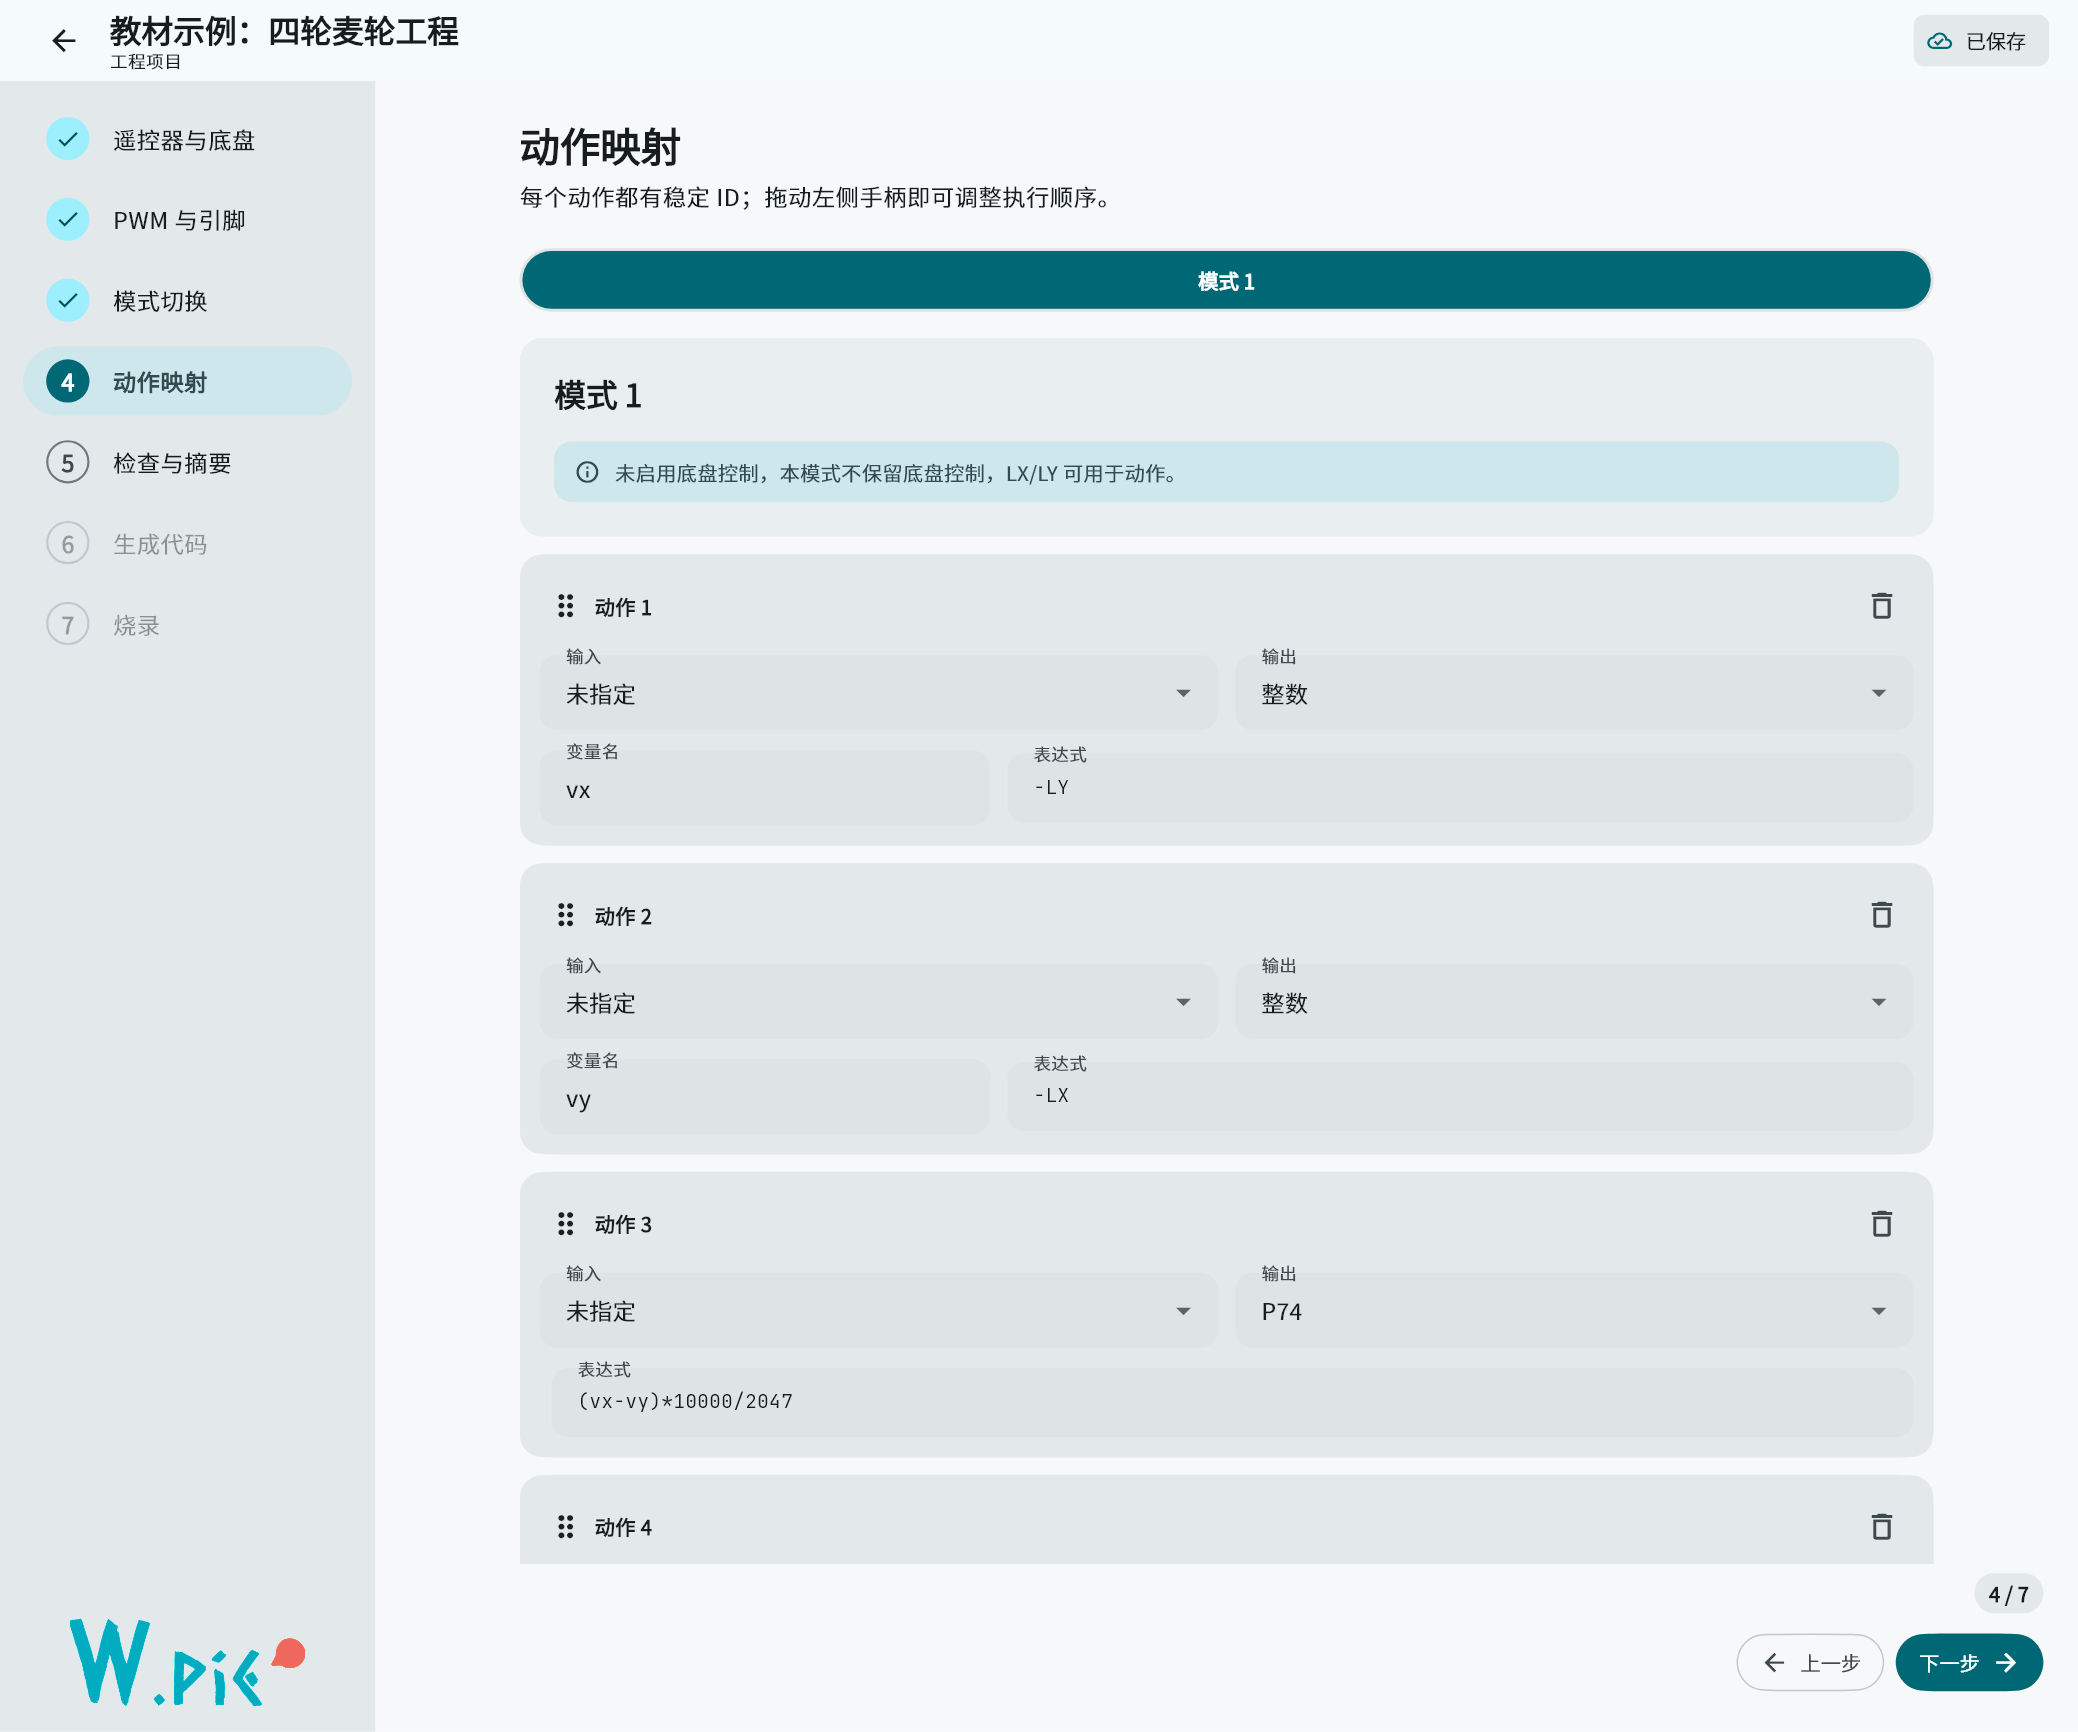
\includegraphics[width=0.86\linewidth]{image/ch05/5-3-mecanum-actions.png}
  \caption{示例 A 的动作映射页（截取前几行）：变量行和车轮表达式}
  \label{fig:ch05-mecanum-actions}
\end{figure}

\paragraph*{检查与试算}
进入“检查与摘要”，检查结果应为 0 错误。表达式行会额外出现“表达式编译
检查”卡片：桌面端可以点“检查表达式”，用内置 SDCC 对生成代码做一次完整
编译，并把错误回填到对应的表达式行；Web 版和 Android 版没有本地编译
流水线，只做解析器校验。旁边的“试算表达式”会打开一个对话框，用滑杆和
按键模拟遥控器输入，按模式顺序执行变量行和表达式行，显示每一行的结果。
它不连接硬件，也不运行生成代码，只用于核对公式。

把“试算表达式”对话框里的 \texttt{LY} 滑杆拖到最左端（$-2047$，等价于摇杆推上）、
其余输入为 0，，
应看到 \texttt{vx=2047}、\texttt{vy=0}，四个轮子都是 10000；把
\texttt{LX} 滑到最左端（$-2047$）、\texttt{LY=0}，应看到 \texttt{vy=2047}，
四个轮子的符号按式~\eqref{eq:ch05-mecanum} 变化。如果某个轮子的符号和你
的接线不一致，先不要改接线，在表达式里把该行整体取反即可
（例如把 \texttt{(vx - vy)} 改成 \texttt{(vy - vx)}）。图~\ref{fig:ch05-mecanum-preview}
是前进满杆时的试算结果。

\begin{figure}[htbp]
  \centering
  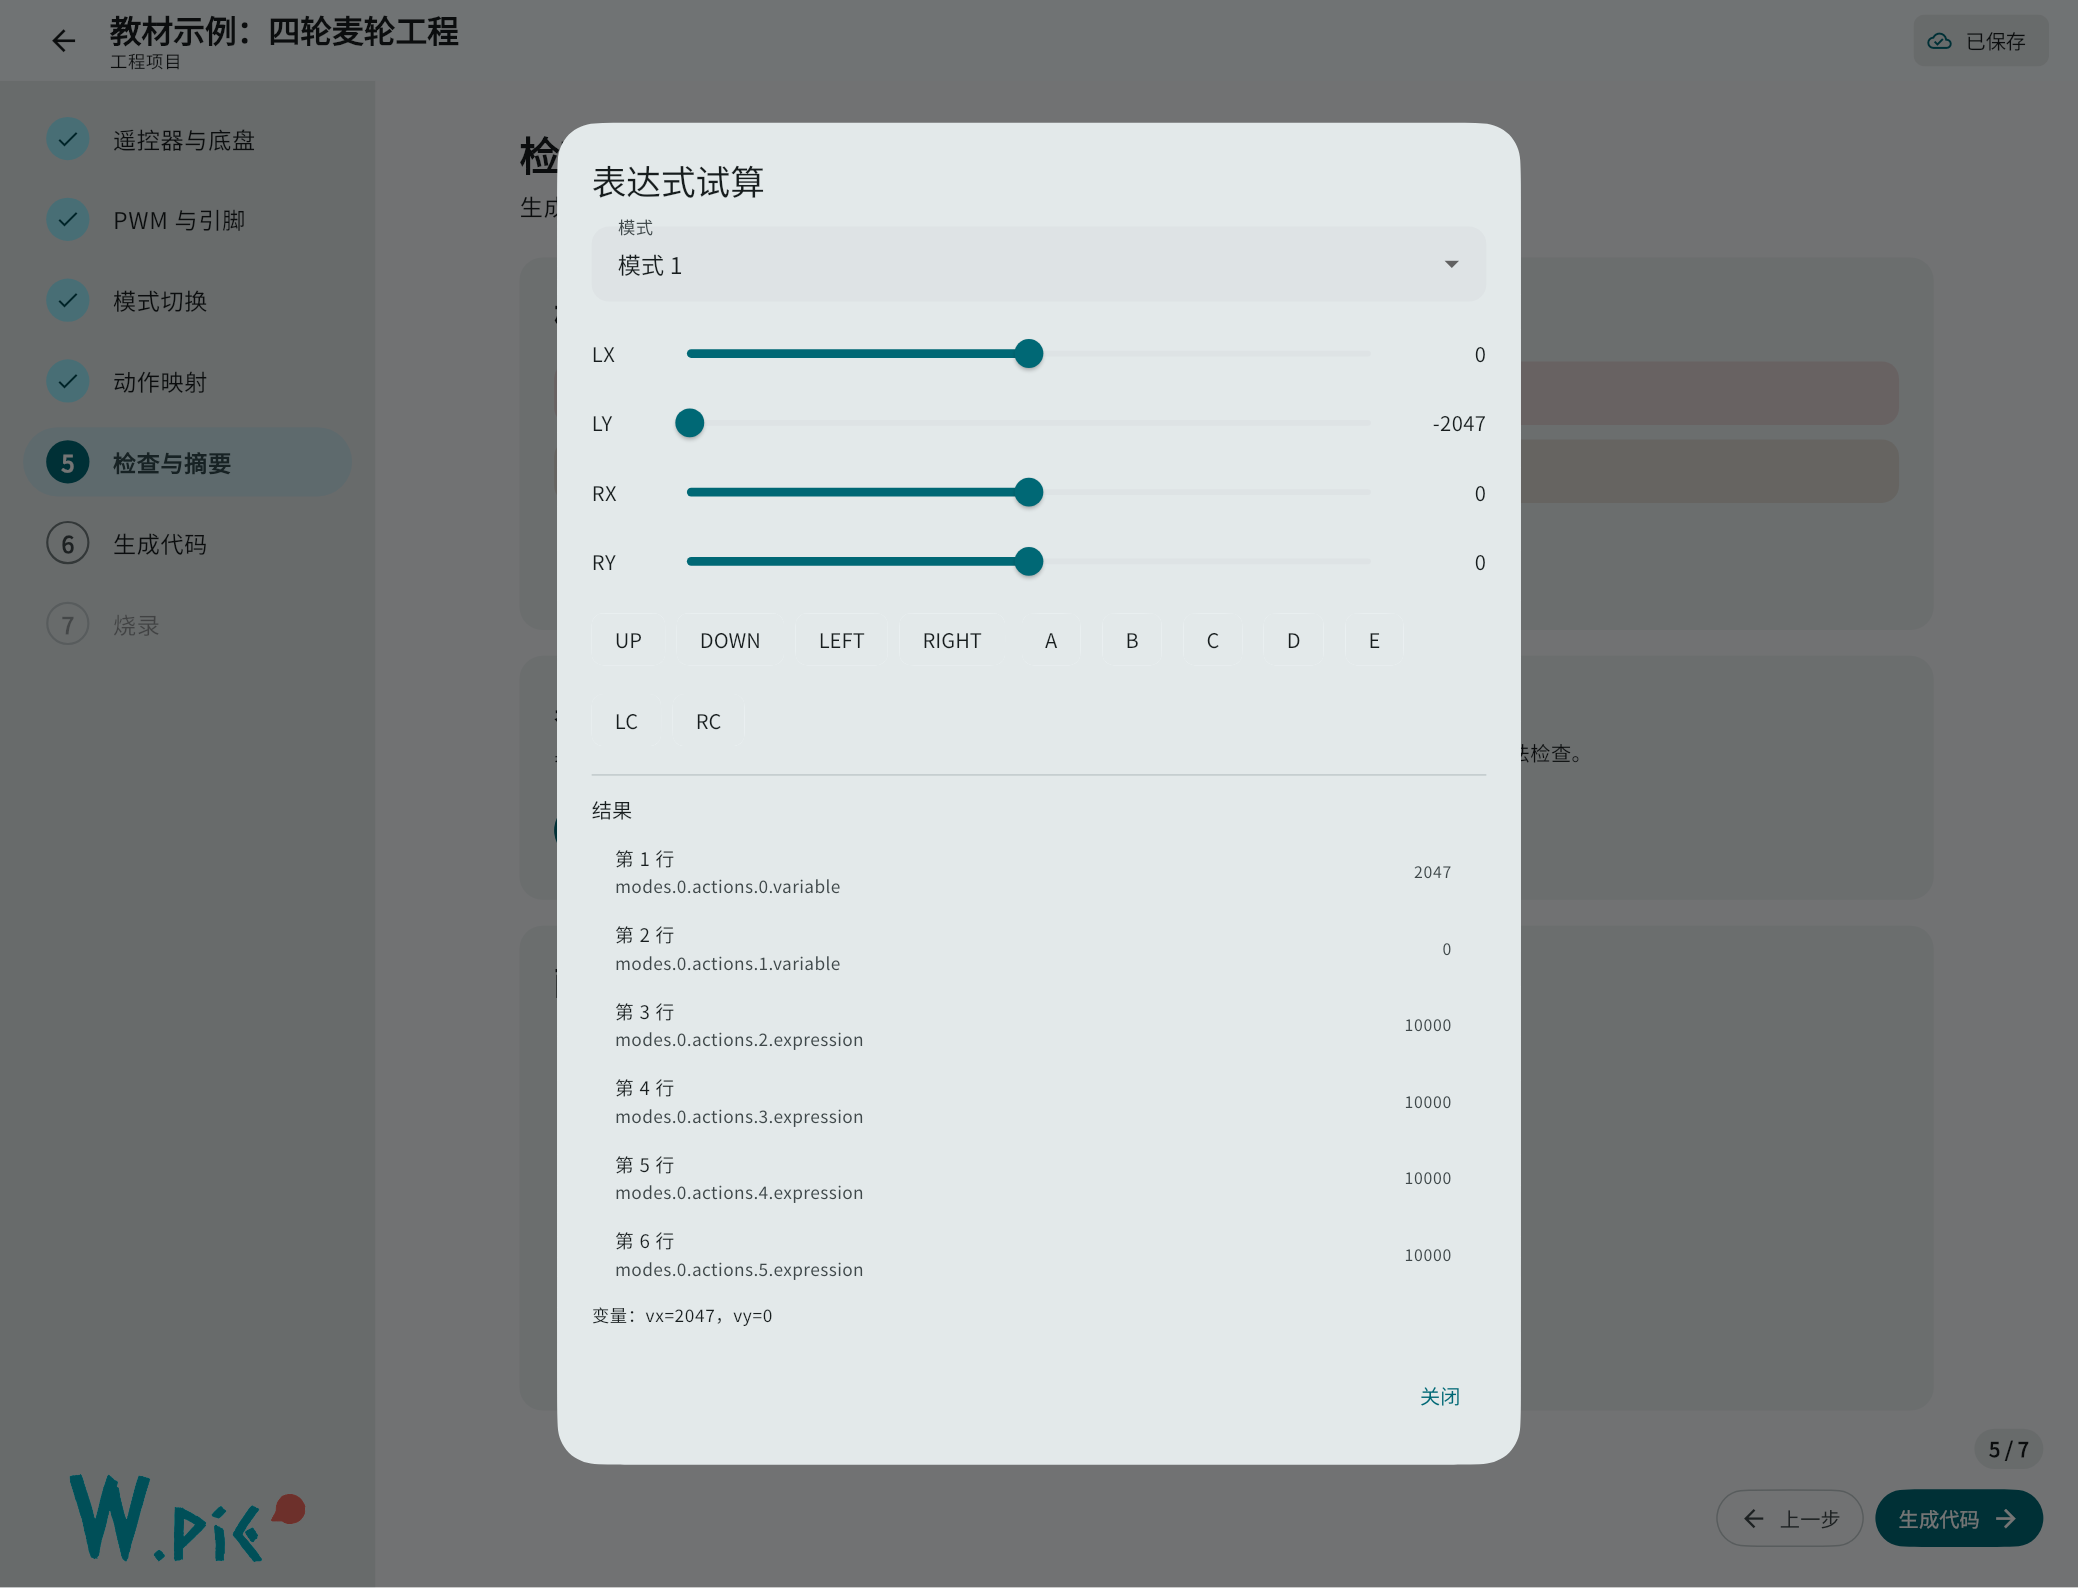
\includegraphics[width=0.84\linewidth]{image/ch05/5-4-mecanum-preview.png}
  \caption{“试算表达式”对话框：\texttt{LY=-2047} 时四个轮子均输出 10000}
  \label{fig:ch05-mecanum-preview}
\end{figure}

\subsection{生成代码与校准}

生成的 \texttt{RunMode1()} 会把变量声明放在函数开头，然后按动作行顺序
赋值。下面是示例 A 的节选（省略了行尾的表达式定位注释）：

\begin{lstlisting}[style=pieblockc,
  caption={示例 A 生成代码的逻辑等价摘录：变量声明与四个轮子的 duty 输出},
  label={lst:ch05-mecanum-c}]
void RunMode1(void)
{
    int32_t pbv_vx = 0;
    int32_t pbv_vy = 0;
    pbv_vx = -valueOfRoker[0][1];             /* -LY */
    pbv_vy = -valueOfRoker[0][0];             /* -LX */
    dutyOfMotor[4] = (int)pb_clamp_i(
        pb_div_i((pbv_vx - pbv_vy) * 10000, 2047), -10000, 10000);
    dutyOfMotor[5] = (int)pb_clamp_i(
        pb_div_i((pbv_vx + pbv_vy) * 10000, 2047), -10000, 10000);
    dutyOfMotor[6] = (int)pb_clamp_i(
        pb_div_i((pbv_vx + pbv_vy) * 10000, 2047), -10000, 10000);
    dutyOfMotor[7] = (int)pb_clamp_i(
        pb_div_i((pbv_vx - pbv_vy) * 10000, 2047), -10000, 10000);
}
\end{lstlisting}

为便于阅读，上面的摘录省去了生成器自动补的显式类型转换，并把除法写成
\texttt{pb\_div\_i}；实际生成代码还会在每行末尾带\texttt{/*@expr:...*/}
定位注释。逻辑与“生成代码”页一致，逐字节代码以页面为准。

这里的 \texttt{dutyOfMotor[4]} 到 \texttt{[7]} 就是 P74--P77 在扩展板
通信协议里的槽位，不是引脚号。变量名加 \texttt{pbv\_} 前缀是生成器做的
命名空间隔离，避免和固件库符号冲突。实际代码以“生成代码”页为准，本书
只摘录关键行。

校准按下面的顺序做，每次只改一个量：

\begin{enumerate}
  \item \textbf{架空}：把车架起来，四轮悬空；遥控器油门保持小值（可以先
        把表达式里的 10000 改成 3000），确认四个轮子都能转、方向可控。
  \item \textbf{单轮方向}：逐个给单轮正 duty，观察轮子转向。若某个轮子
        反了，把该行的表达式整体取反，不要改接线，方便以后对照。
  \item \textbf{前后}：推左摇杆向上，四个轮子应同时向前；若后退，把
        \texttt{vx} 的表达式从 \texttt{-LY} 改成 \texttt{LY}。
  \item \textbf{左右}：推左摇杆向左，车应向左平移；若向右，把
        \texttt{vy} 的表达式从 \texttt{-LX} 改成 \texttt{LX}。
  \item \textbf{斜向}：四角各推一次，观察是否往正确的对角方向走。若某个
        对角方向走反，通常是对角两个轮子的符号同时错了，回到第 2 步逐个
        核对。
  \item \textbf{落地}：架空确认后落地，先用低速度走直线和横移，再逐步
        提高速度；注意电流、电调和电机温度。
\end{enumerate}

\begin{note}
表达式行直接写 duty 真值，应用层没有软件斜坡。上电、模式切换或从 0 直接
推到满杆时，输出可能是阶跃。电机电调本身可能有软启动，但不能依赖它。
第一次调试务必架空、限速，并确保车前方没有人。
\end{note}

\subsection{边界：麦轮能做到什么，不能做到什么}

麦轮混控在本工具里是“开环 + 固定缩放”的：

\begin{itemize}
  \item 没有编码器回读，轮速与地面速度的对应关系靠标定和电池电压维持；
  \item 没有陀螺仪，自转只能用开环 \texttt{RX} 近似，会漂移；
  \item 式~\eqref{eq:ch05-duty} 的固定缩放不能同时保证所有方向的线性度，
        对角线满杆会饱和；需要更平滑的特性时，可以用 \texttt{max/abs}
        在表达式里做每轮动态归一化，但表达式会明显变长；
  \item 麦轮对地面、轮子磨损和辊子方向很敏感，四个轮子新旧不一致时会
        跑偏；这是机械问题，不是表达式能完全补偿的。
\end{itemize}

\section{全向轮}

\subsection{90$^\circ$ 辊子与切向力}

全向轮（Omni wheel）的轮缘周围装着轴线与轮子轴线成 $90^\circ$ 的小辊子；
辊子轴线落在轮子平面内，所以轮子只能沿滚动方向出力。
轮子转动时只能沿自身前进方向出力；垂直于轮子方向的分量会让辊子自由滚动，
几乎不产生阻力。因此全向轮没有麦轮那种斜向分力，必须靠多个轮子的方向
组合来合成平移。

图~\ref{fig:ch05-omni} 左侧是单个全向轮：沿轮子方向可以驱动，侧向可以
自由滑动；右侧是三轮 120$^\circ$ 布局。三个轮子的滚动方向互成
120$^\circ$，它们的速度组合就能覆盖平面内任意平移方向。三轮布局结构
简单、成本低，但对重心位置和轮子接地压力比较敏感；四轮全向轮更稳，
但需要处理其中一个轮子可能悬空的问题。

\begin{figure}[htbp]
  \centering
  \begin{minipage}{0.44\linewidth}
    \centering
    \begin{tikzpicture}[scale=0.9,>=Latex,font=\small,
      wheel/.style={draw=black!60,fill=gray!10,line width=0.9pt},
      roller/.style={draw=black!45,line width=0.5pt},
      axis/.style={-{Latex[length=2mm]},line width=1pt,structurecolor},
      lab/.style={font=\small,inner sep=1pt}]
      % 轮子侧视：滚动方向在纸面内，主轴垂直于纸面
      \draw[wheel] (0,0) circle (1.5);
      \foreach \a in {15,45,...,345} {
        \draw[roller] (\a:1.2) -- (\a:1.63);
        \draw[fill=gray!35,draw=black!45] (\a:1.63) circle (0.10);
      }
      % 主轴：垂直纸面的三维示意（双箭头 + 端面椭圆）
      \draw[<->,line width=0.9pt,structurecolor] (-0.58,-0.40) -- (0.58,0.40);
      \draw[fill=white,draw=structurecolor,line width=0.7pt]
        [rotate around={34:(-0.58,-0.40)}] (-0.58,-0.40) ellipse (0.20 and 0.07);
      \draw[fill=white,draw=structurecolor,line width=0.7pt]
        [rotate around={34:(0.58,0.40)}] (0.58,0.40) ellipse (0.20 and 0.07);
      \node[lab,structurecolor] at (0.72,0.30) {主轴};
      % 驱动方向：轮心速度，沿接触点切线（水平）
      \draw[axis] (0,0) -- (2.6,0) node[right] {可驱动};
      % 地面与接触点
      \draw[black!50,line width=0.7pt] (-1.9,-1.5) -- (1.9,-1.5);
      \foreach \gx in {-1.75,-1.45,...,1.75} {
        \draw[black!35] (\gx,-1.5) -- (\gx-0.14,-1.66); }
      \fill[black] (0,-1.5) circle (1.5pt);
      \node[lab,align=center] at (0,-2.06)
        {单轮侧视：辊子轴线与主轴成 $90^\circ$\\双箭头为主轴，垂直纸面；
        侧向可沿主轴自由滚动};
    \end{tikzpicture}
  \end{minipage}\hfill
  \begin{minipage}{0.50\linewidth}
    \centering
    \begin{tikzpicture}[scale=0.9,>=Latex,font=\small,
      axis/.style={-{Latex[length=2mm]},line width=1pt,structurecolor},
      wheel/.style={draw=black!65,fill=gray!15,rounded corners=1.5pt,line width=0.7pt},
      lab/.style={font=\small,inner sep=1pt}]
      \draw[dashed,black!35] (0,0) circle (1.65);
      \draw[fill=structurecolor!6,draw=structurecolor!60] (0,0) circle (0.48);
      \foreach \a/\n/\pos in {0/1/above right,120/2/above right,240/3/below left} {
        \draw[axis] (0,0) -- (\a:2.45) node[\pos] {$v_{\n}$};
        \draw[wheel,rotate around={\a:(\a:1.65)}]
          (\a:1.65) ++(-0.42,-0.16) rectangle ++(0.84,0.32);
      }
      \draw[axis,dashed] (0,0) -- (3.2,0) node[right] {$x$};
      \draw[axis,dashed] (0,0) -- (0,3.2) node[above] {$y$};
    \end{tikzpicture}
  \end{minipage}
  \caption{全向轮：单轮侧视（左，滚动方向在纸面内，侧向可沿主轴自由滚动，
  主轴垂直于纸面）与三轮 120$^\circ$ 滚动方向（右）}
  \label{fig:ch05-omni}
\end{figure}

真实的全向轮如图~\ref{fig:ch05-photo-omni} 所示：辊子的轴线与主轴成
$90^\circ$，侧向受力时辊子绕自身轴线自由滚动，几乎不产生阻力。

\begin{figure}[htbp]
  \centering
  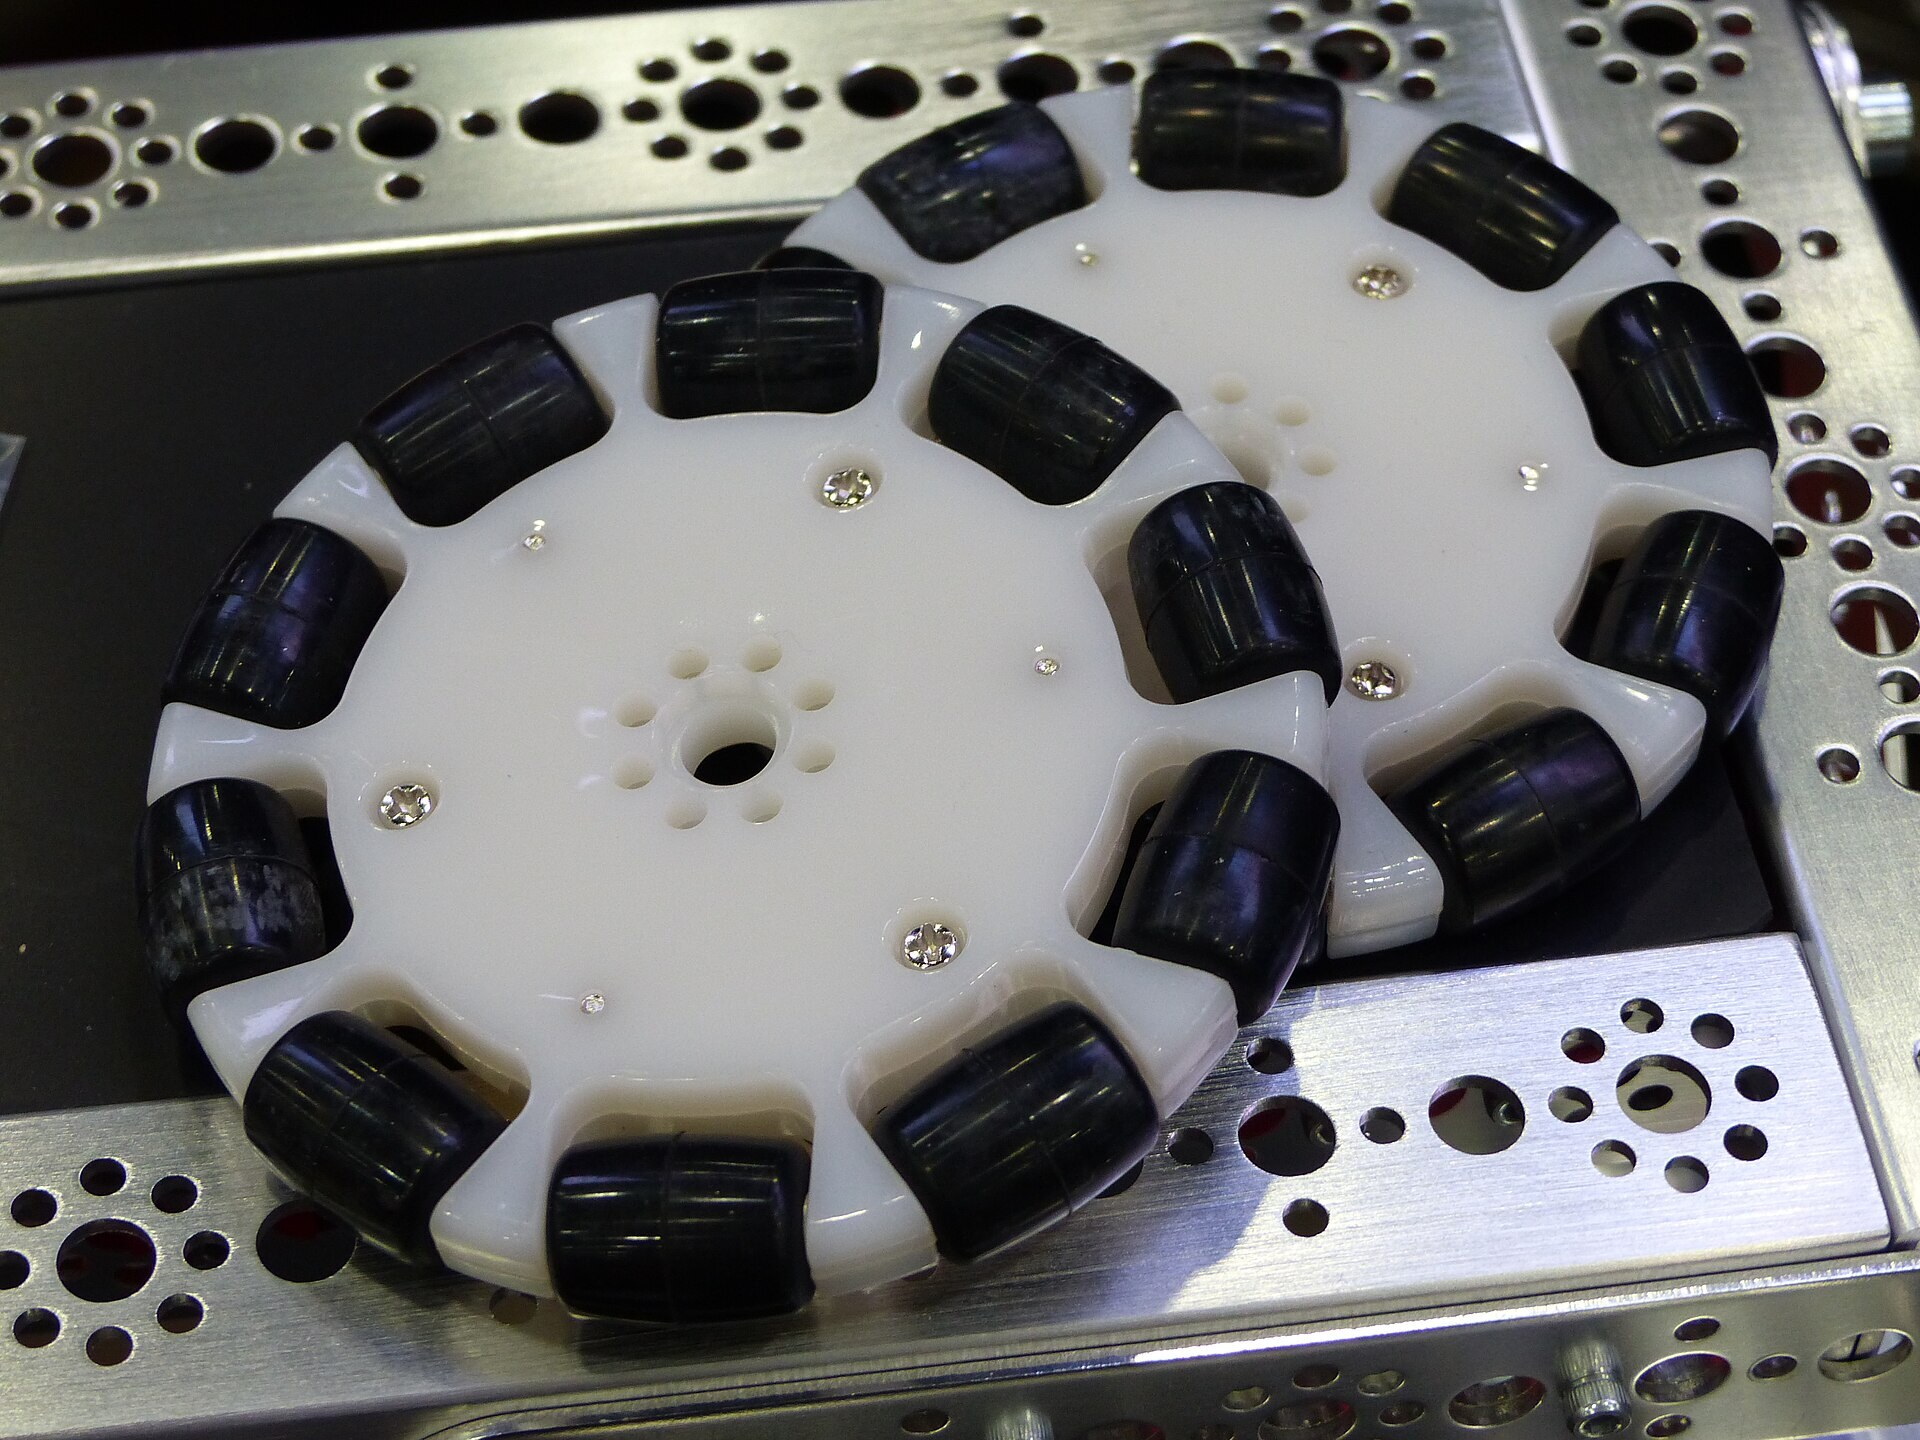
\includegraphics[width=0.74\linewidth]{image/ch05/photo-omni.jpg}
  \caption{真实的全向轮：辊子轴线与主轴垂直（成 $90^\circ$），侧向可自由
  滚动（照片：Stilfehler，Wikimedia Commons，CC BY-SA 4.0）}
  \label{fig:ch05-photo-omni}
\end{figure}

\subsection{三轮 120$^\circ$ 运动学}

把第 $i$ 个轮子的滚动方向与 $x$ 轴的夹角记为 $\phi_i$，忽略自转时：

\begin{equation}
v_i = v_x\cos\phi_i + v_y\sin\phi_i.
\label{eq:ch05-omni}
\end{equation}

取 $\phi_1=0^\circ$、$\phi_2=120^\circ$、$\phi_3=240^\circ$：

\begin{equation}
\begin{aligned}
v_1 &= v_x, \\
v_2 &= -\tfrac12 v_x + \tfrac{\sqrt3}{2} v_y, \\
v_3 &= -\tfrac12 v_x - \tfrac{\sqrt3}{2} v_y.
\end{aligned}
\label{eq:ch05-omni3}
\end{equation}

$\sqrt3/2\approx0.866$。三个轮子的 duty 仍按式~\eqref{eq:ch05-duty}
换算和钳位。注意这里的 $\phi_i$ 是\textbf{滚动方向}，不是轮子在车体上的
安装位置角；图~\ref{fig:ch05-omni} 右侧标的是滚动方向。实际装配时，
如果某个轮子的滚动方向与图示相反，把该轮的符号取反即可。

\subsection{示例 A2：三轮全向工程车}

三轮全向的配置步骤与示例 A 相同，只改三处：

\begin{enumerate}
  \item PWM 与引脚：P74、P75、P76 设为“平滑电机”，P77 以及
        P60/P62/P64/P66 设为“未使用”；PWMA 50\,Hz，PWMB 10000\,Hz。
  \item 动作映射：前两行仍然是 \texttt{vx = -LY}、\texttt{vy = -LX}，
        后三行按表~\ref{tab:ch05-omni-rows} 填写。
  \item 检查与试算：\texttt{LY=-2047}、其余为 0 时，轮 1 为 10000，
        轮 2、轮 3 为 $-5000$；\texttt{LX=-2047} 时，轮 1 为 0，
        轮 2 为正、轮 3 为负。
\end{enumerate}

\begin{table}[htbp]
  \centering
  \small
  \setlength{\tabcolsep}{4pt}
  \begin{tabularx}{\linewidth}{@{}c l l >{\raggedright\arraybackslash}X l@{}}
    \toprule
    行 & 输出 & 变量名 & 表达式 & 轮子 \\
    \midrule
    3 & P74 & — & \texttt{vx * 10000 / 2047} & 1，$\phi=0^\circ$ \\
    4 & P75 & — & \texttt{(-0.5 * vx + 0.866 * vy) * 10000 / 2047} & 2，$\phi=120^\circ$ \\
    5 & P76 & — & \texttt{(-0.5 * vx - 0.866 * vy) * 10000 / 2047} & 3，$\phi=240^\circ$ \\
    \bottomrule
  \end{tabularx}
  \caption{三轮全向示例的动作行（前两行同表~\ref{tab:ch05-mecanum-rows}）}
  \label{tab:ch05-omni-rows}
\end{table}

\subsection{麦轮与全向轮的对比}

两种构型的差异如表~\ref{tab:ch05-omni-compare} 所示。

\begin{table}[H]
  \centering
  \small
  \begin{tabularx}{\linewidth}{@{}l >{\raggedright\arraybackslash}X >{\raggedright\arraybackslash}X@{}}
    \toprule
    对比项 & 麦克纳姆轮 & 全向轮 \\
    \midrule
    辊子角度 & 与轮子轴线约 $45^\circ$ & 与轮子轴线约 $90^\circ$ \\
    力的方向 & 斜向分力，四轮合成 & 仅沿滚动方向，多轮合成 \\
    常见轮数 & 4 & 3 或 4 \\
    平移 & 四轮混控 & 三轮/四轮混控 \\
    自转 & 四轮差速，容易 & 三轮需要额外布局，四轮较容易 \\
    优点 & 效率较高、四轮承载稳 & 结构简单、成本低、侧向阻力小 \\
    缺点 & 辊子磨损/地面敏感、斜向力复杂 & 三轮接地压力敏感、承载较小 \\
    本工具支持 & 关底盘 + 表达式，有示例 & 关底盘 + 表达式，有示例 \\
    \bottomrule
  \end{tabularx}
  \caption{麦克纳姆轮与全向轮的主要差异}
  \label{tab:ch05-omni-compare}
\end{table}

\section{舵轮}

\subsection{模块结构}

舵轮（Swerve module）把“转向”和“驱动”做成两个独立自由度：一个舵机
（或转向电机）带动轮子绕竖直轴转向，另一个电机驱动轮子前进或后退。
四个舵轮模块就能让车体在不改变车头朝向的情况下，向任意方向平移，并且
可以原地自转。它的抓地力、越障能力和效率通常优于麦轮，但每个模块都
需要转向角反馈、零位标定和限位保护，成本和调试量都高得多。

图~\ref{fig:ch05-steering} 左侧是单个模块的俯视示意：转向轴在轮子中心，
舵机把轮子转到 $\beta$ 角，驱动电机让轮子以速度 $s$ 沿轮子朝向滚动；右侧是
四个模块以同一转向角 $\beta$ 转向的布局，此时车头朝向不变，整车沿斜向
平移。每个模块的转向角和驱动速度都要根据车体运动指令单独计算，不能像
麦轮那样只靠四个轮子的线性组合。

\begin{figure}[htbp]
  \centering
  \begin{minipage}{0.46\linewidth}
    \centering
    \begin{tikzpicture}[scale=0.9,>=Latex,font=\small,
      body/.style={draw=structurecolor!70,fill=structurecolor!6,
        rounded corners=3pt,line width=0.9pt},
      wheel/.style={draw=black!65,fill=gray!15,
        rounded corners=2pt,line width=0.8pt},
      axis/.style={-{Latex[length=2mm]},line width=0.9pt,structurecolor},
      lab/.style={font=\small,inner sep=1pt}]
      % 坐标系与图 5.3 一致：x 向前（页面向上），y 向左（页面向左）
      \draw[body] (-2.6,-2.2) rectangle (2.2,2.6);
      \draw[axis] (0,0) -- (0,3.3) node[above] {$x$};
      \draw[axis] (0,0) -- (-3.0,0) node[left] {$y$};
      % 转向平台 + 轮子：自 x 轴向 y 轴（左）转过 beta=40 度，
      % 轮胎面垂直于滚动方向
      \begin{scope}[rotate=130]
        \draw[draw=black!45,fill=gray!6,rounded corners=2pt,line width=0.6pt]
          (-1.05,-0.55) rectangle (1.05,0.55);
        \draw[wheel] (-1.5,-0.28) rectangle (1.5,0.28);
        \foreach \t in {-1.25,-0.95,...,1.25} {
          \draw[black!40,line width=0.5pt] (\t,-0.28) -- (\t,0.28); }
      \end{scope}
      % 转向轴（画在最上层）
      \draw[fill=white,draw=black!50] (0,0) circle (0.5);
      \draw[black!50] (-0.32,0) -- (0.32,0);
      \draw[black!50] (0,-0.32) -- (0,0.32);
      % 标注：舵机负责转向，驱动电机装在转向平台上随轮子转向
      \node[lab,align=center] at (1.45,1.7) {舵机\\（转向）};
      \draw[black!50,->] (1.2,1.42) -- (0.44,0.44);
      \node[lab,anchor=west] at (0.72,-1.72) {驱动电机};
      \draw[black!50,->] (0.9,-1.56) -- (0.64,-0.82);
      \node[lab,anchor=east] at (-0.78,-1.42) {转向轴};
      \draw[black!50,->] (-0.72,-1.34) -- (-0.4,-0.42);
      % beta 角弧与驱动速度 s
      \draw[->,black!65] (0,1.85) arc[start angle=90,end angle=130,radius=1.85];
      \node[lab] at (112:2.12) {$\beta$};
      \draw[axis] (130:1.9) -- (130:2.8) node[above left] {$s$};
    \end{tikzpicture}
  \end{minipage}\hfill
  \begin{minipage}{0.48\linewidth}
    \centering
    \begin{tikzpicture}[scale=0.78,>=Latex,font=\small,
      body/.style={draw=structurecolor!70,fill=structurecolor!6,
        rounded corners=3pt,line width=0.9pt},
      wheel/.style={draw=black!65,fill=gray!15,
        rounded corners=1.5pt,line width=0.7pt},
      axis/.style={-{Latex[length=2mm]},line width=0.9pt,structurecolor},
      lab/.style={font=\small,inner sep=1pt}]
      \draw[body] (-2.7,-2.0) rectangle (2.7,2.0);
      % 四个模块同转向角（30 度）：蟹行平移
      \foreach \x/\y in {-2.0/1.45, 2.0/1.45, -2.0/-1.45, 2.0/-1.45} {
        \begin{scope}[shift={(\x,\y)},rotate=30]
          \draw[wheel] (-0.28,-0.95) rectangle (0.28,0.95);
          \foreach \t in {-0.65,-0.25,0.15,0.55} {
            \draw[black!40,line width=0.5pt] (-0.28,\t) -- (0.28,\t); }
        \end{scope}
        \draw[black!50] (\x,\y) circle (0.10);
      }
      \draw[axis] (0,0) -- (30:3.3) node[right] {$v$};
      \node[lab,below] at (0,-2.3) {四模块同转向角：车头不变，斜向平移};
    \end{tikzpicture}
  \end{minipage}
  \caption{舵轮：单模块的转向角与驱动（左）和四模块同角转向的斜向平移（右）}
  \label{fig:ch05-steering}
\end{figure}

\subsection{模块运动学}

设车体指令为 $(v_x,v_y,\omega)$，第 $i$ 个模块的安装位置为
$(x_i,y_i)$，则该模块轮心的目标速度为：

\begin{equation}
v_{x,i}=v_x-\omega y_i,\qquad v_{y,i}=v_y+\omega x_i.
\label{eq:ch05-swerve-velocity}
\end{equation}

转向角与驱动速度分别为：

\begin{equation}
\beta_i=\operatorname{atan2}(v_{y,i},v_{x,i}),\qquad
s_i=\sqrt{v_{x,i}^2+v_{y,i}^2}.
\label{eq:ch05-swerve-angle}
\end{equation}

舵机的角度范围通常只有 $\pm90^\circ$，而 $\beta_i$ 来自 \texttt{atan2}，
范围是 $\pm180^\circ$。工程上的标准处理是“角度回绕 + 驱动反向”：

\begin{equation}
\beta_i\leftarrow
\begin{cases}
\beta_i-180^\circ, & \beta_i>90^\circ,\\
\beta_i+180^\circ, & \beta_i<-90^\circ,
\end{cases}
\quad s_i\leftarrow -s_i.
\label{eq:ch05-swerve-wrap}
\end{equation}

这样每个模块的舵机只需要在 $\pm90^\circ$ 内转动，轮子正反转由驱动电机
负责。再叠加每个模块的零位偏移和安装方向，才是最终下发角度。没有转向
角回读时，零位靠机械限位或外部工装标定，上电后必须缓慢回到零位，不能
直接给大角度指令。

\subsection{为什么本期不做舵轮}

从引脚数量看，四个模块需要 4 路驱动 + 4 路转向，正好占满 8 路扩展输出：
P74--P77 设 10000\,Hz 驱动，P60、P62、P64、P66 设 50\,Hz 转向。主控板还有 MP03、
MP74 两个主舵机口，可以留给两自由度机械臂或其他小机构；但 8 路扩展输出
已经占满，不能再接云台、拨弹或摩擦轮，整机扩展性很差。

更关键的是软件能力。PIE-Block 没有“舵轮模块”这个配置对象，也没有
模块零位、限位、方向、转向角回读的界面；生成代码不会做
式~\eqref{eq:ch05-swerve-angle} 的计算，也不会处理式~\eqref{eq:ch05-swerve-wrap}
的回绕。表达式系统理论上可以手工拼出四个模块的公式：每个模块用
\texttt{atan2} 和 \texttt{sqrt} 算出 $\beta_i$ 与 $s_i$，再分别写舵机和
电机输出；四模块大约需要 24 行。但这属于“用户自己写控制律”，没有内建
校验、没有标定流程，也没有经过验证的示例，本章不把它列为支持能力。

\begin{note}
如果你在比赛方案里必须用舵轮，建议把舵轮控制放到独立的自定义固件里，
用带编码器的转向电机做闭环，再通过主控板 CAN/串口接收速度指令；
不要把四模块开环舵轮当作 PIE-Block 的“高级配置”直接上场。
\end{note}

\section{机械臂逆解}

\subsection{正解与逆解}

机械臂的正运动学（forward kinematics）是“已知每个关节角，求末端执行器
的位置”；逆运动学（inverse kinematics，IK）是反过来，“已知末端要去的
位置，求每个关节应该转到什么角度”。PIE-Block 的表达式只能算右值，没有
循环和迭代，因此本章只讨论\textbf{闭式解}：用代数公式直接算出关节角，
不做数值迭代。

二自由度平面臂是最小的教学例子：两个连杆 $L_1$、$L_2$ 在同一平面内，
肩关节在原点，末端目标是 $(x,y)$。它有两个解：肘上（elbow-up）和肘下
（elbow-down）。逆解还要处理可达性：目标太远或太近时，公式里的
$\cos q_2$ 会超出 $[-1,1]$，必须钳位；否则会出现无效角度或数值异常。

图~\ref{fig:ch05-arm-ik} 是二连杆的几何关系。实线是肘下解，虚线是同一
目标点的肘上解；两个虚线圆之间是可达的工作空间，内圆半径
$|L_1-L_2|$，外圆半径 $L_1+L_2$。

\begin{figure}[htbp]
  \centering
  \begin{tikzpicture}[scale=0.95,>=Latex,font=\small,
    link/.style={line width=2.2pt,structurecolor},
    linkd/.style={line width=1.2pt,black!55,dashed},
    axis/.style={-{Latex[length=2.2mm]},line width=0.8pt,black!70},
    dim/.style={black!40,dashed,line width=0.6pt},
    lab/.style={font=\small,inner sep=1.5pt}]
    % 工作空间
    \draw[dim] (0,0) circle (5.2);
    \draw[dim] (0,0) circle (0.8);
    % 坐标轴
    \draw[axis] (-0.6,0) -- (6.2,0) node[right] {$x$};
    \draw[axis] (0,-0.6) -- (0,6.0) node[above] {$y$};
    % 肘上解
    \coordinate (O) at (0,0);
    \coordinate (E1) at (2.955,0.516);
    \coordinate (T) at (3.218,2.700);
    \draw[link] (O) -- (E1) -- (T);
    \fill[structurecolor] (O) circle (2pt);
    \fill[structurecolor] (E1) circle (2pt);
    \fill[black] (T) circle (2pt);
    % 肘下解
    \coordinate (E2) at (1.021,2.820);
    \draw[linkd] (O) -- (E2) -- (T);
    \fill[black!55] (E2) circle (1.8pt);
    % 目标标注
    \node[lab,right] at (T) {$(x,y)$};
    \node[lab,below] at (O) {肩关节 $O$};
    \node[lab] at (2.05,0.62) {$L_1$};
    \node[lab,right] at (3.10,1.62) {$L_2$};
    % q1 角弧
    \draw[->,black!65] (1.05,0) arc[start angle=0,end angle=9.9,radius=1.05];
    \node[lab] at (1.42,0.45) {$q_1$};
    % q2 角弧（在肘关节处，从 L1 延长线到 L2）
    \draw[->,black!65] ($(E1)+(9.9:0.72)$) arc[start angle=9.9,end angle=83.2,radius=0.72];
    \node[lab] at ($(E1)+(45:0.95)$) {$q_2$};
    % 内外圆标注
    \node[lab] at (4.55,0.55) {$L_1+L_2$};
    \node[lab] at (0.15,1.05) {$|L_1-L_2|$};
    % 图例
  \node[lab,anchor=north west] at (-0.4,-1.35)
    {实线：肘下解；虚线：肘上解};
  \end{tikzpicture}
  \caption{二连杆机械臂的几何关系：实线为肘下解（$s_2>0$），虚线为肘上解
  （$s_2<0$）；两个虚线圆之间为可达工作空间}
  \label{fig:ch05-arm-ik}
\end{figure}

\subsection{二连杆公式}

记目标到肩关节的距离平方为 $r^2=x^2+y^2$，由余弦定理：

\begin{equation}
c_2=\frac{r^2-L_1^2-L_2^2}{2L_1L_2}.
\label{eq:ch05-ik-c2}
\end{equation}

实际计算前先把 $c_2$ 钳位到 $[-1,1]$，记为 $\tilde c_2$，再取

\begin{equation}
s_2=\sqrt{1-\tilde c_2^2}.
\label{eq:ch05-ik-s2}
\end{equation}

这里的 $s_2\ge0$ 对应肘下解（肘关节落在肩—目标连线的下方，见
图~\ref{fig:ch05-arm-ik} 的实线）；取负号就是肘上解。两个关节角为：

\begin{equation}
q_2=\operatorname{atan2}(s_2,\tilde c_2),\qquad
q_1=\operatorname{atan2}(y,x)-\operatorname{atan2}(L_2s_2,\,L_1+L_2\tilde c_2).
\label{eq:ch05-ik-angles}
\end{equation}

$\operatorname{atan2}(y,x)$ 的参数顺序是“先 $y$ 后 $x$”，不是“先 $x$ 后
$y$”。这一点在 C 的 \texttt{atan2}、Dart 的 \texttt{atan2} 和本书公式里
都一致；写表达式时不要写反。

可达工作空间是

\begin{equation}
|L_1-L_2|\le\sqrt{x^2+y^2}\le L_1+L_2.
\label{eq:ch05-ik-workspace}
\end{equation}

目标在工作空间外时，钳位会把关节角推到边界，机器人会“够不到但停在边界”，
不会报错。这既是一种保护，也意味着操作者不能只看公式，还要看机械限位和
实际姿态。目标在奇异点附近（完全伸直或完全折叠）时，关节角的微小变化
可能对应末端较大的运动，速度要放慢。

\subsection{示例 B：二自由度机械臂}

\paragraph*{硬件假设}
肩关节舵机接 MP03，肘关节舵机接 MP74；两个都是主控板上的 50\,Hz 主舵机
口。连杆长度 $L_1=120$\,mm、$L_2=100$\,mm；两个舵机的中位都设为
$0^\circ$。机械臂安装在车体前方，臂平面竖直；目标 $(x,y)$ 以肩关节为
原点，$x$ 向前、$y$ 向上。示例只在前上方工作：$x\ge20$\,mm、
$y\ge0$\,mm，避免肩关节解落到 $\pm90^\circ$ 之外。

\paragraph*{输入映射}
右摇杆控制目标：右推（\texttt{RX} 正）增大 $x$，上推（\texttt{RY} 负）
增大 $y$。比例取 $0.05$\,mm/计数，满杆约 $\pm102$\,mm：

\begin{equation}
x=\max(0.05\cdot\texttt{RX},\,20),\qquad
y=\max(-0.05\cdot\texttt{RY},\,0).
\label{eq:ch05-arm-input}
\end{equation}

两个 $\max$ 把目标限制在安全的前上象限，也避免 $x=0$ 时
$\operatorname{atan2}(y,x)$ 在原点附近跳变。代价是摇杆推到左下时目标
停在下边界，而不是真的走到车体后方；这是有意的取舍。

\paragraph*{动作行}
按表~\ref{tab:ch05-arm-rows} 添加 10 行。前 8 行输出“有理数”变量，
最后两行输出 MP03、MP74。变量必须按顺序定义：\texttt{c2} 用到
\texttt{r2}，\texttt{s2} 用到 \texttt{c2c}，\texttt{q1} 用到
\texttt{s2} 和 \texttt{c2c}，所以不能打乱行序。

\begin{table}[htbp]
  \centering
  \small
  \setlength{\tabcolsep}{4pt}
  \begin{tabularx}{\linewidth}{@{}c l l l >{\raggedright\arraybackslash}X l@{}}
    \toprule
    行 & 输入 & 输出 & 变量名 & 表达式 & 说明 \\
    \midrule
    1 & 未指定 & 有理数 & \texttt{x} & \texttt{max(RX * 0.05, 20.0)} & 前向距离 \\
    2 & 未指定 & 有理数 & \texttt{y} & \texttt{max(-RY * 0.05, 0.0)} & 高度 \\
    3 & 未指定 & 有理数 & \texttt{r2} & \texttt{x * x + y * y} & 距离平方 \\
    4 & 未指定 & 有理数 & \texttt{c2} & \texttt{(r2 - 24400.0) / 24000.0} & 余弦定理 \\
    5 & 未指定 & 有理数 & \texttt{c2c} & \texttt{min(max(c2, -1.0), 1.0)} & 可达性钳位 \\
    6 & 未指定 & 有理数 & \texttt{s2} & \texttt{sqrt(1.0 - c2c * c2c)} & 肘上解 \\
    7 & 未指定 & 有理数 & \texttt{q1} & \texttt{atan2(y, x) - atan2(100.0 * s2, 120.0 + 100.0 * c2c)} & 肩关节角 \\
    8 & 未指定 & 有理数 & \texttt{q2} & \texttt{atan2(s2, c2c)} & 肘关节角 \\
    9 & 未指定 & MP03 & — & \texttt{q1 * 180.0 / PI} & 肩舵机角度 \\
    10 & 未指定 & MP74 & — & \texttt{q2 * 180.0 / PI - 90.0} & 肘舵机角度 \\
    \bottomrule
  \end{tabularx}
  \caption{示例 B 的动作行：8 行变量加 2 行舵机输出}
  \label{tab:ch05-arm-rows}
\end{table}

表~\ref{tab:ch05-arm-rows} 里的常数来自 $L_1=120$、$L_2=100$：
$L_1^2+L_2^2=24400$，$2L_1L_2=24000$。肘舵机在直臂时 $q_2=0$，指令
$0-90=-90^\circ$；完全折叠时 $q_2=180^\circ$，指令 $90^\circ$。如果你的
机械臂直臂时舵机中位不是 $-90^\circ$，把最后一行的 $-90.0$ 改成你的零位
偏置，而不是只改页面上的“中位°”。

\begin{note}
表达式行输出到舵机时，角度是\textbf{绝对角度}：$0^\circ$ 对应 1.5\,ms，
$+90^\circ$ 对应 2.5\,ms，$-90^\circ$ 对应 0.5\,ms。页面上的“中位°”只在
初始化时使用，不会叠加到表达式结果上。示例把中位设为 0，机械零位直接写
在表达式里。上电后第一个主循环就会用表达式结果覆盖初始值，所以机械臂
可能立刻动一下；上电前必须支撑好机械臂，并留出运动空间。
\end{note}

图~\ref{fig:ch05-arm-actions} 和图~\ref{fig:ch05-arm-servos} 是动作映射页
的上、下两部分。变量行的表达式较长，输入框里可能只显示开头；完整的式子
以表~\ref{tab:ch05-arm-rows} 为准。

\begin{figure}[H]
  \centering
  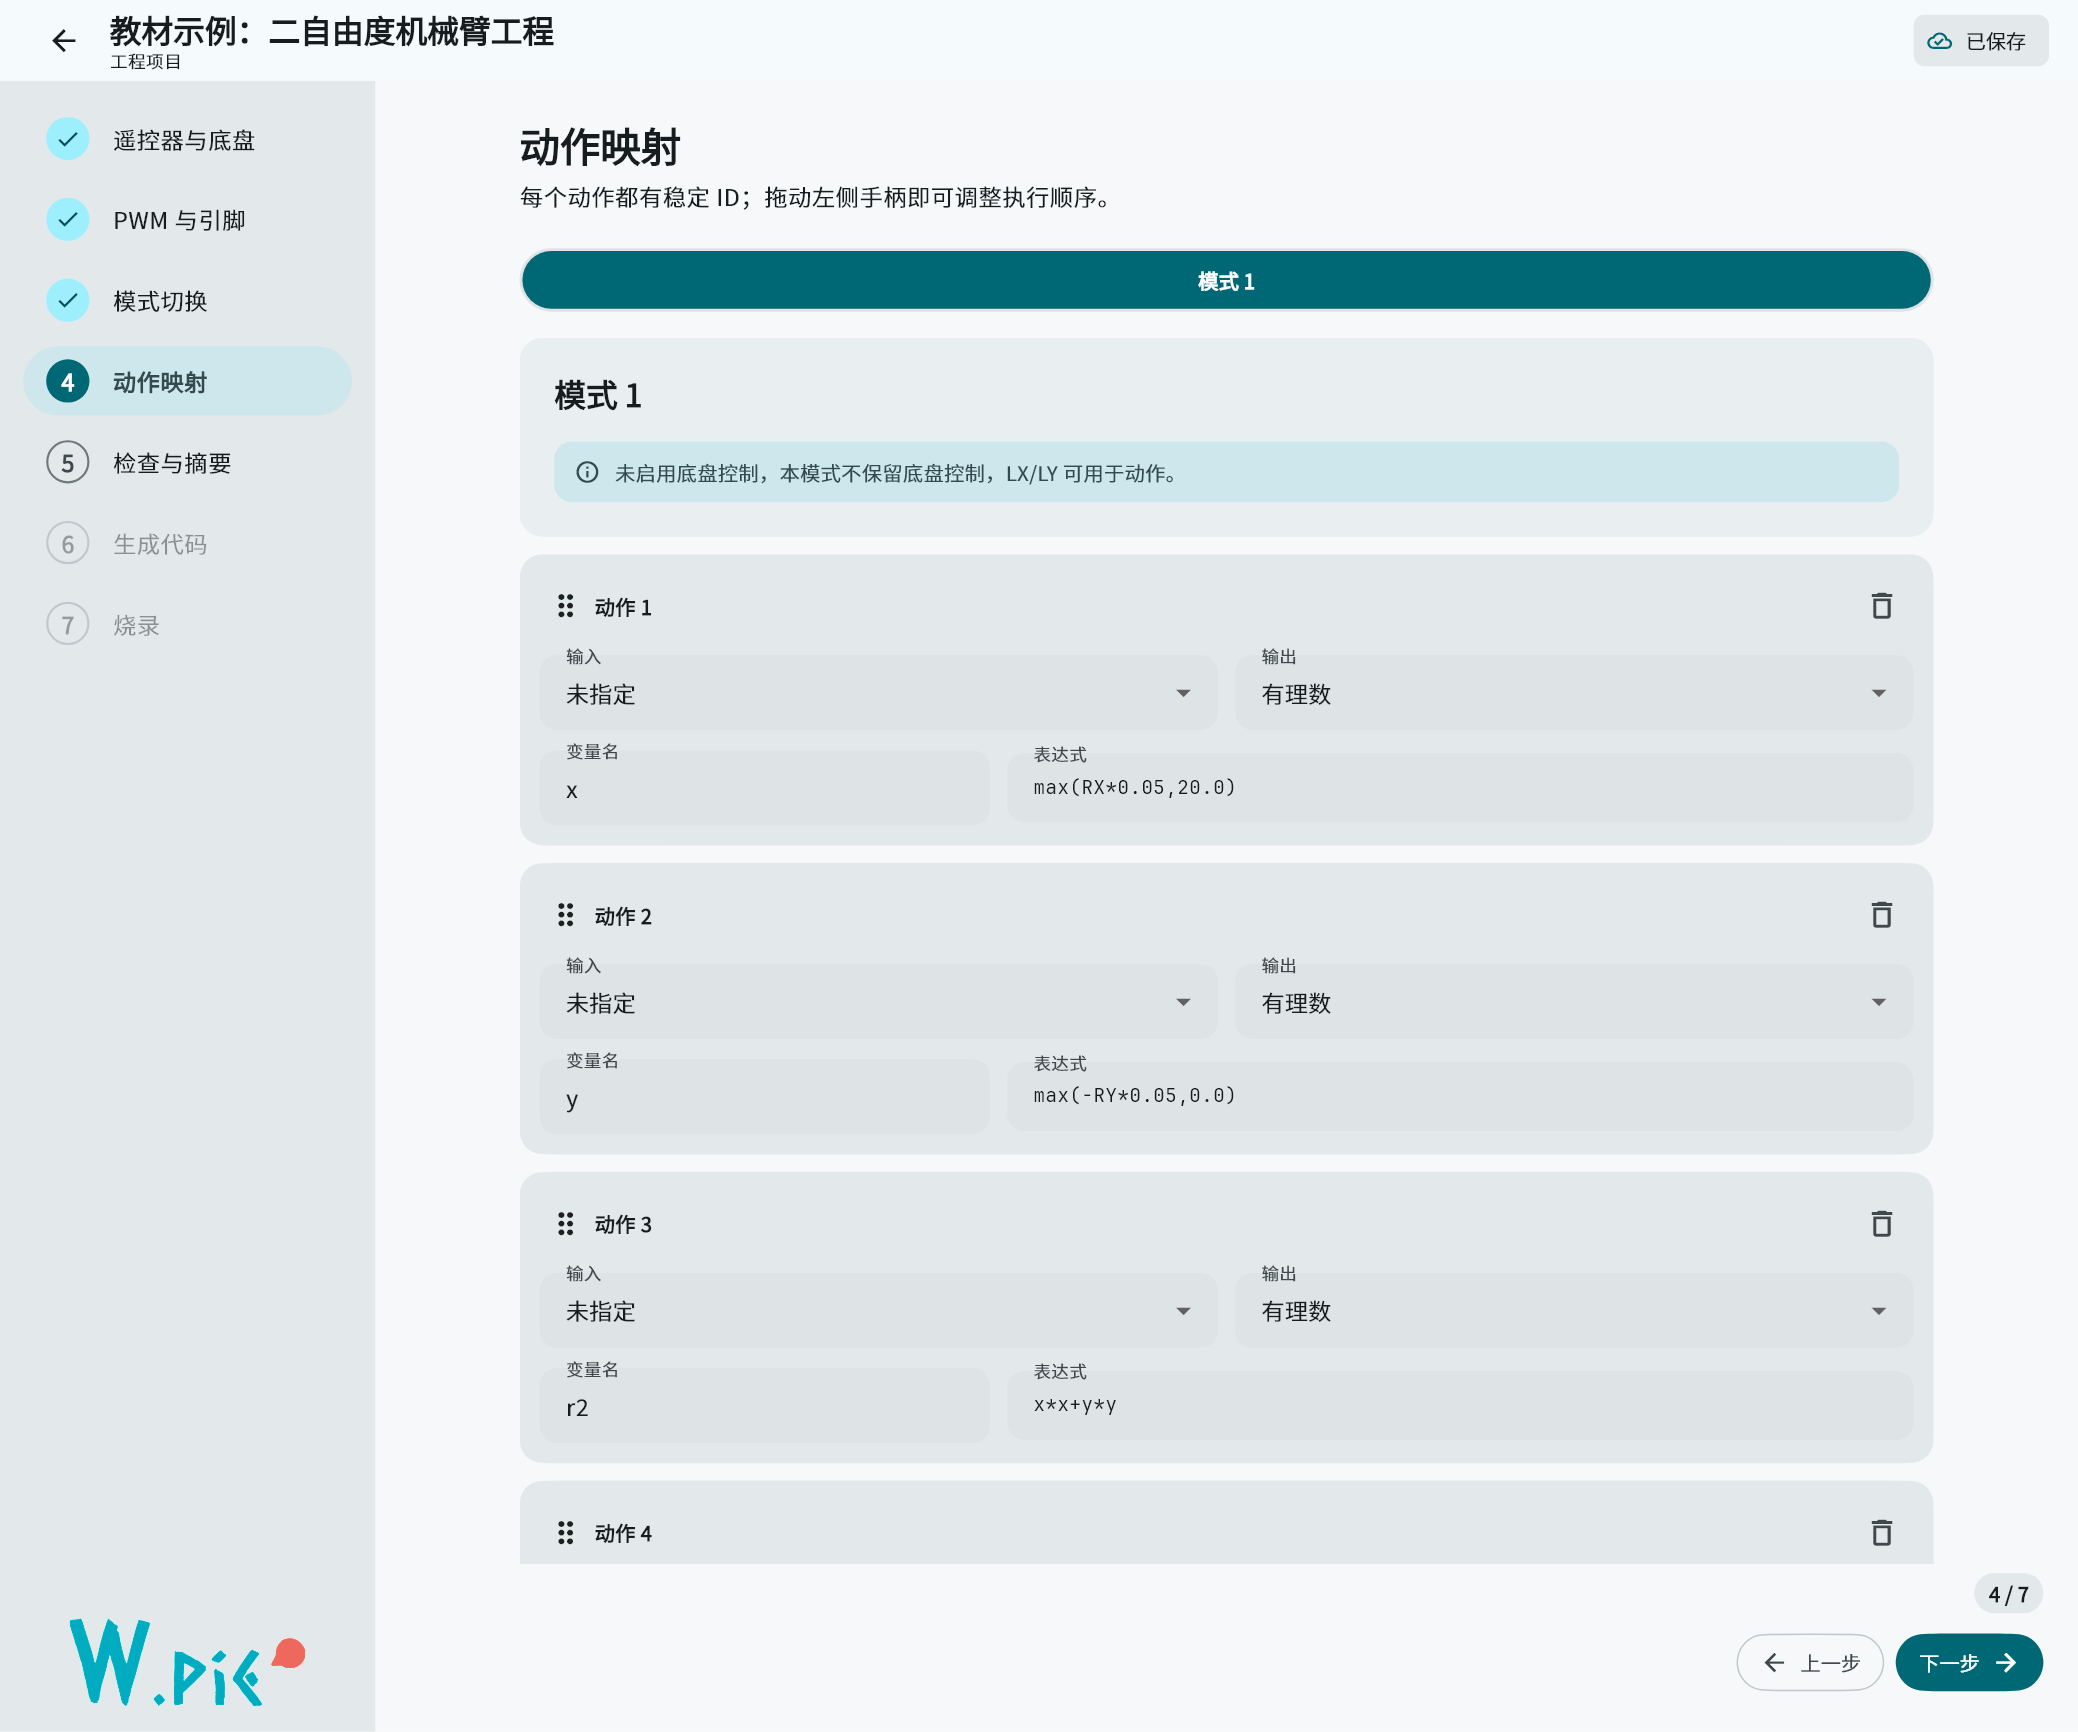
\includegraphics[width=0.86\linewidth]{image/ch05/5-5-arm-actions.png}
  \caption{示例 B 的动作映射页上半部分：用变量行把逆解拆成中间量}
  \label{fig:ch05-arm-actions}
\end{figure}

\paragraph*{试算与检查}
打开“试算表达式”，把 \texttt{RX} 设成 1023、\texttt{RY} 设成 $-1023$，
应看到 $x=y\approx51.15$，\texttt{q1} 约 $-11.3^\circ$，\texttt{q2} 约
$143.0^\circ$，肩/肘指令约 $-11.3^\circ/53.0^\circ$，都在 $\pm90^\circ$
内。再把 \texttt{RX}、\texttt{RY} 推到四个角，确认所有输出都落在
$-90^\circ$ 到 $+90^\circ$ 之间；如果某个角越界，说明你的工作空间或零位
需要调整。

桌面端可以点“检查表达式”，让 SDCC 真正编译一次生成代码，确认
\texttt{sqrt}/\texttt{atan2} 和浮点运行时能通过。表达式编译通过不等于
实机安全：它只证明语法、类型和 C 代码能编译，不证明你的机械参数、
舵机方向和工作空间正确。

\begin{lstlisting}[style=pieblockc,
  caption={示例 B 生成代码的逻辑等价摘录：逆解与两个主舵机的角度输出},
  label={lst:ch05-arm-c}]
void RunMode1(void)
{
    float pbv_x = 0.0f, pbv_y = 0.0f, pbv_r2 = 0.0f, pbv_c2 = 0.0f;
    float pbv_c2c = 0.0f, pbv_s2 = 0.0f, pbv_q1 = 0.0f, pbv_q2 = 0.0f;
    pbv_x = pb_max_f(RX * 0.05f, 20.0f);
    pbv_y = pb_max_f(-RY * 0.05f, 0.0f);
    pbv_r2 = pbv_x * pbv_x + pbv_y * pbv_y;
    pbv_c2 = pb_div_f(pbv_r2 - 24400.0f, 24000.0f);
    pbv_c2c = pb_min_f(pb_max_f(pbv_c2, -1.0f), 1.0f);
    pbv_s2 = pb_sqrt(1.0f - pbv_c2c * pbv_c2c);
    pbv_q1 = pb_atan2(pbv_y, pbv_x)
           - pb_atan2(100.0f * pbv_s2, 120.0f + 100.0f * pbv_c2c);
    pbv_q2 = pb_atan2(pbv_s2, pbv_c2c);
    mainServoDuty[0] = pb_servo_duty(
        pb_clamp_f(pbv_q1 * 57.29578f, -90.0f, 90.0f));
    mainServoDuty[1] = pb_servo_duty(
        pb_clamp_f(pbv_q2 * 57.29578f - 90.0f, -90.0f, 90.0f));
}
\end{lstlisting}

同样，这段代码省去了自动生成的显式类型转换，并保留了生成器的
\texttt{pb\_div\_f}/\texttt{pb\_div\_i} 调用；\texttt{57.29578} 是
$180/\pi$ 的近似值，生成器实际写成“乘 180 再除以 \texttt{PI}”。关键是
两条：变量按顺序声明和赋值，舵机输出前统一钳位到 $\pm90^\circ$。

\begin{figure}[H]
  \centering
  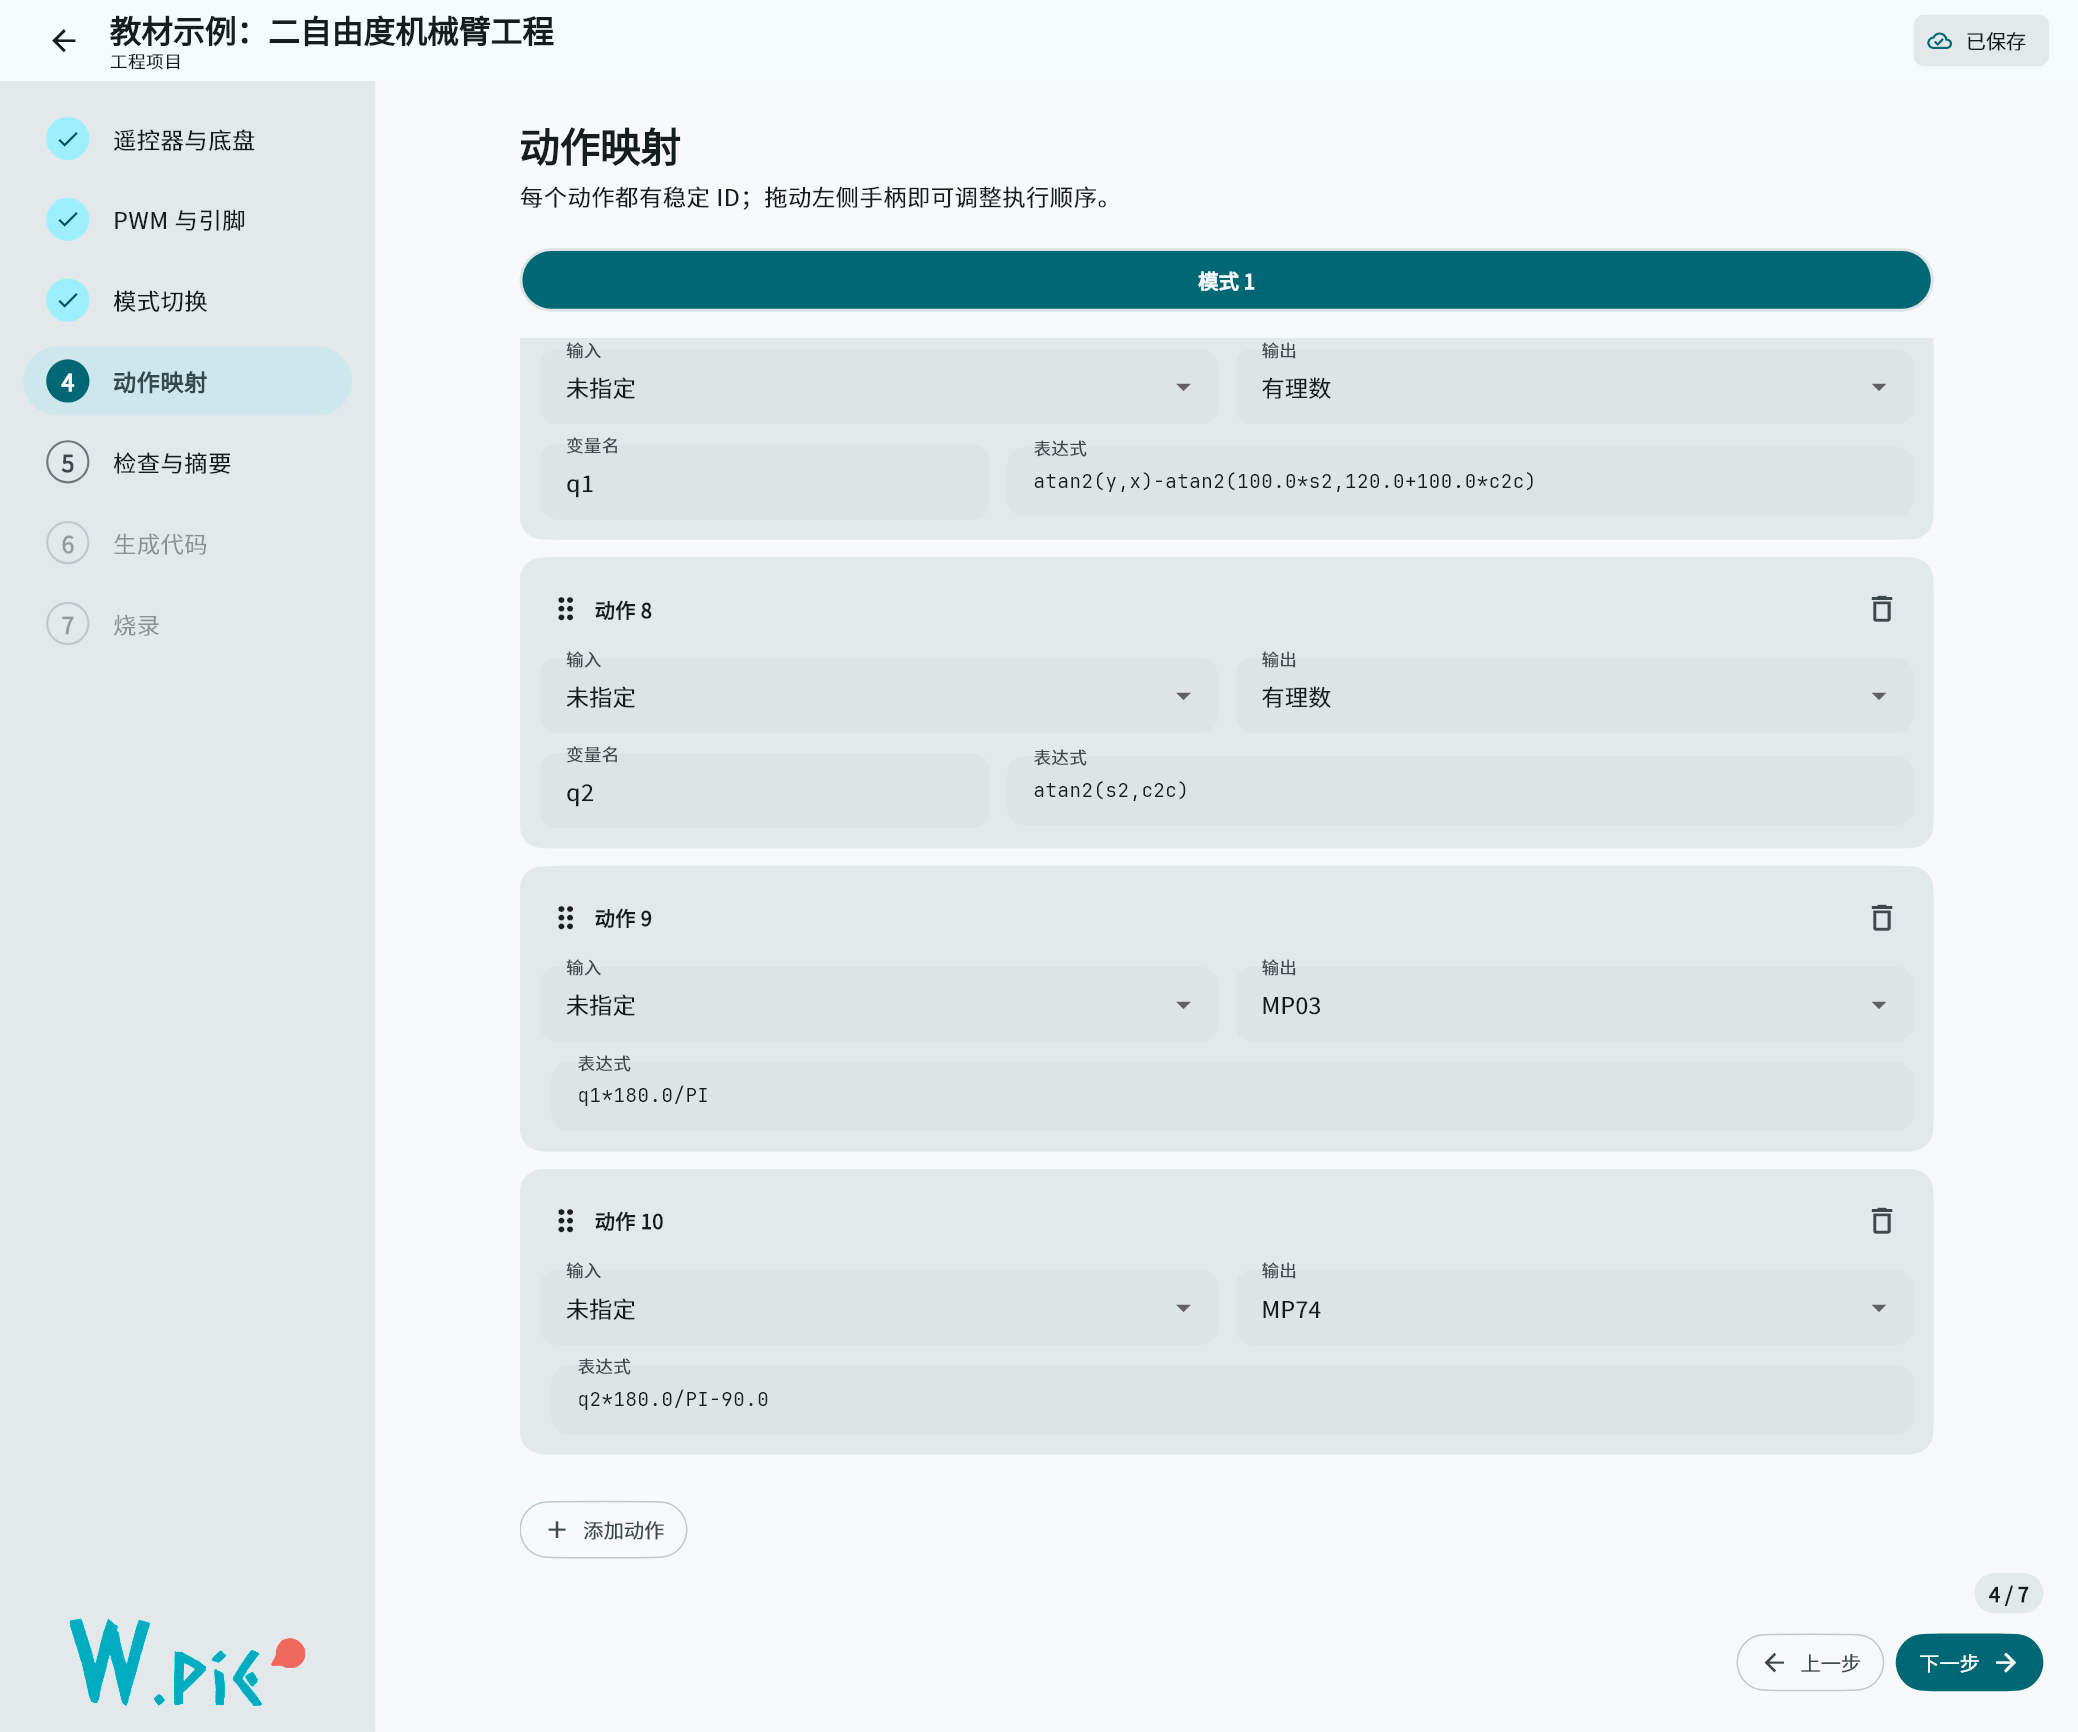
\includegraphics[width=0.86\linewidth]{image/ch05/5-6-arm-servos.png}
  \caption{示例 B 的动作映射页下半部分：\texttt{q1/q2} 和两个主舵机输出}
  \label{fig:ch05-arm-servos}
\end{figure}

\subsection{舵机零位、方向与限位}

机械臂的精度最终取决于机械零位和舵机方向，而不是公式。建议按以下顺序
标定：

\begin{enumerate}
  \item 拆下连杆或让机械臂悬空，给肩、肘舵机分别发 $0^\circ$，记录舵盘
        位置；把舵盘装到你定义的机械零位。
  \item 给肩舵机发 $-20^\circ$、$+20^\circ$，确认正方向与公式一致；
        若相反，在肩舵机表达式前加负号。
  \item 给肘舵机发 $-90^\circ$、$-45^\circ$、$0^\circ$，确认直臂、半弯、
        全弯的方向；若相反，把最后一行的 \texttt{q2 * 180.0 / PI - 90.0}
        改成 \texttt{90.0 - q2 * 180.0 / PI}。
  \item 在机械限位内逐步扩大角度，记录会碰到结构的位置，用
        \texttt{min/max} 把指令夹在安全范围内，例如
        \texttt{min(max(q1 * 180.0 / PI, -60.0), 60.0)}。
  \item 装回连杆，先让目标在远离奇异点的工作空间中心附近小范围移动，
        再扩大范围；全程低速、有人扶住急停。
\end{enumerate}

\begin{note}
舵机没有位置回读。表达式算出的角度是“命令角度”，不是“实际角度”。
连杆间隙、舵机死区、电池电压和负载都会让实际角偏离命令值。不要用
开环机械臂做需要精确重复定位的任务；抓取和放置要留机械容差。
\end{note}

\subsection{三自由度及以上}

三自由度的常见形式是“底座偏航 + 平面二连杆”。如果底座偏航角由另一个
舵机控制，而目标 $(x,y)$ 是在\textbf{机械臂局部平面}里给出的，那么平面
二连杆的公式完全不变，只是多了一个底座舵机。如果目标是在\textbf{车体
世界坐标}里给出的，需要先把目标绕底座旋转到局部坐标：

\begin{equation}
\begin{aligned}
x' &= x\cos\beta+y\sin\beta,\\
y' &= -x\sin\beta+y\cos\beta.
\end{aligned}
\label{eq:ch05-arm-rotate}
\end{equation}

式~\eqref{eq:ch05-arm-rotate} 需要 \texttt{sin/cos}，而当前表达式白名单
只有 \texttt{abs}、\texttt{min}、\texttt{max}、\texttt{sign}、
\texttt{sqrt}、\texttt{atan2} 和常量 \texttt{PI/E}，没有 \texttt{sin/cos}。
因此“底座旋转 + 世界坐标目标”在当前工具里不能直接写；
可以改用局部坐标摇杆（目标相对臂平面给出），或者另立需求为表达式增加
三角函数。不要用多项式近似硬凑，精度和可维护性都不划算。

四自由度及以上、六自由度数值逆解、轨迹规划和闭环控制都不在当前能力
范围内。原因不是“表达式不够长”，而是缺少循环、矩阵、状态和反馈；
即使勉强写出，20\,ms 周期、可用代码区约 64\,KB Flash 和开环机械结构也无法保证效果。

\section{修改、组合与排错}

\subsection{常用修改}

表~\ref{tab:ch05-edits} 列出最常见的修改。每次只改一处，改完用试算
核对，再生成代码。

\begin{table}[htbp]
  \centering
  \small
  \begin{tabularx}{\linewidth}{@{}l >{\raggedright\arraybackslash}X >{\raggedright\arraybackslash}X@{}}
    \toprule
    目的 & 改哪里 & 例子 \\
    \midrule
    单个电机反向 & 该轮表达式整体取反 & \texttt{(vx - vy)} 改为 \texttt{(vy - vx)} \\
    整车限速 & 把 10000 改小 & \texttt{* 6000 / 2047} \\
    前后反向 & \texttt{vx} 的符号 & \texttt{-LY} 改为 \texttt{LY} \\
    左右反向 & \texttt{vy} 的符号 & \texttt{-LX} 改为 \texttt{LX} \\
    加开环自转 & 四条轮表达式加 \texttt{RX} 项 & 左前/左后 \texttt{- RX}，右前/右后 \texttt{+ RX}（符号按式~\eqref{eq:ch05-mecanum-yaw}，幅值先小后大） \\
    改连杆长度 & 改 IK 的四个常数 & $L_1=150,L_2=120$：24400→36900，24000→36000，100.0→120.0，120.0→150.0 \\
    改舵机零位 & 舵机表达式加常数 & \texttt{q1 * 180.0 / PI + 5.0} \\
    限制关节角 & 用 \texttt{min/max} 夹住 & \texttt{min(max(q1 * 180.0 / PI, -60.0), 60.0)} \\
    \bottomrule
  \end{tabularx}
  \caption{常见修改及对应的表达式改法}
  \label{tab:ch05-edits}
\end{table}

\subsection{编辑流程}

推荐把“改程序”当成一个闭环，而不是改完就烧：

\begin{enumerate}
  \item 在动作映射页修改一行表达式或变量名；
  \item 到检查页看错误/警告，点“试算表达式”核对典型输入；
  \item 桌面端点“检查表达式”，确认生成代码能通过 SDCC；
  \item 到生成代码页看 \texttt{RunMode1()}，确认变量顺序和输出行符合预期；
  \item 编译、烧录；架空低速测试；确认后再落地。
\end{enumerate}

生成代码页是只读的。不要直接改 \texttt{main.c} 再编译，因为下一次生成会
把它覆盖；所有修改都应该回到配置里。项目文件自动保存，停止输入约 0.5\,s
后就会写入；如果不确定是否保存，看右上角的“已保存”状态。

\subsection{把麦轮和机械臂合到一辆车上}

示例 A 和示例 B 可以合到同一个工程项目里：四个麦轮仍然接 P74--P77，
PWMB 设 10000\,Hz；两个主舵机接 MP03、MP74，PWMA 设 50\,Hz。动作行按
下面的顺序放在同一个模式里：

\begin{enumerate}
  \item 麦轮的 \texttt{vx}、\texttt{vy} 两行；
  \item 四个车轮表达式；
  \item 机械臂的 \texttt{x}、\texttt{y}、\texttt{r2}、\texttt{c2}、
        \texttt{c2c}、\texttt{s2}、\texttt{q1}、\texttt{q2} 八行；
  \item 两个舵机表达式。
\end{enumerate}

图~\ref{fig:ch05-photo-arm} 就是这样一台“麦轮底盘 + 舵机机械臂”的教学
机器人：底盘负责全向移动，机械臂负责抓取，与示例 A、示例 B 合并后的构型
思路一致。

\begin{figure}[htbp]
  \centering
  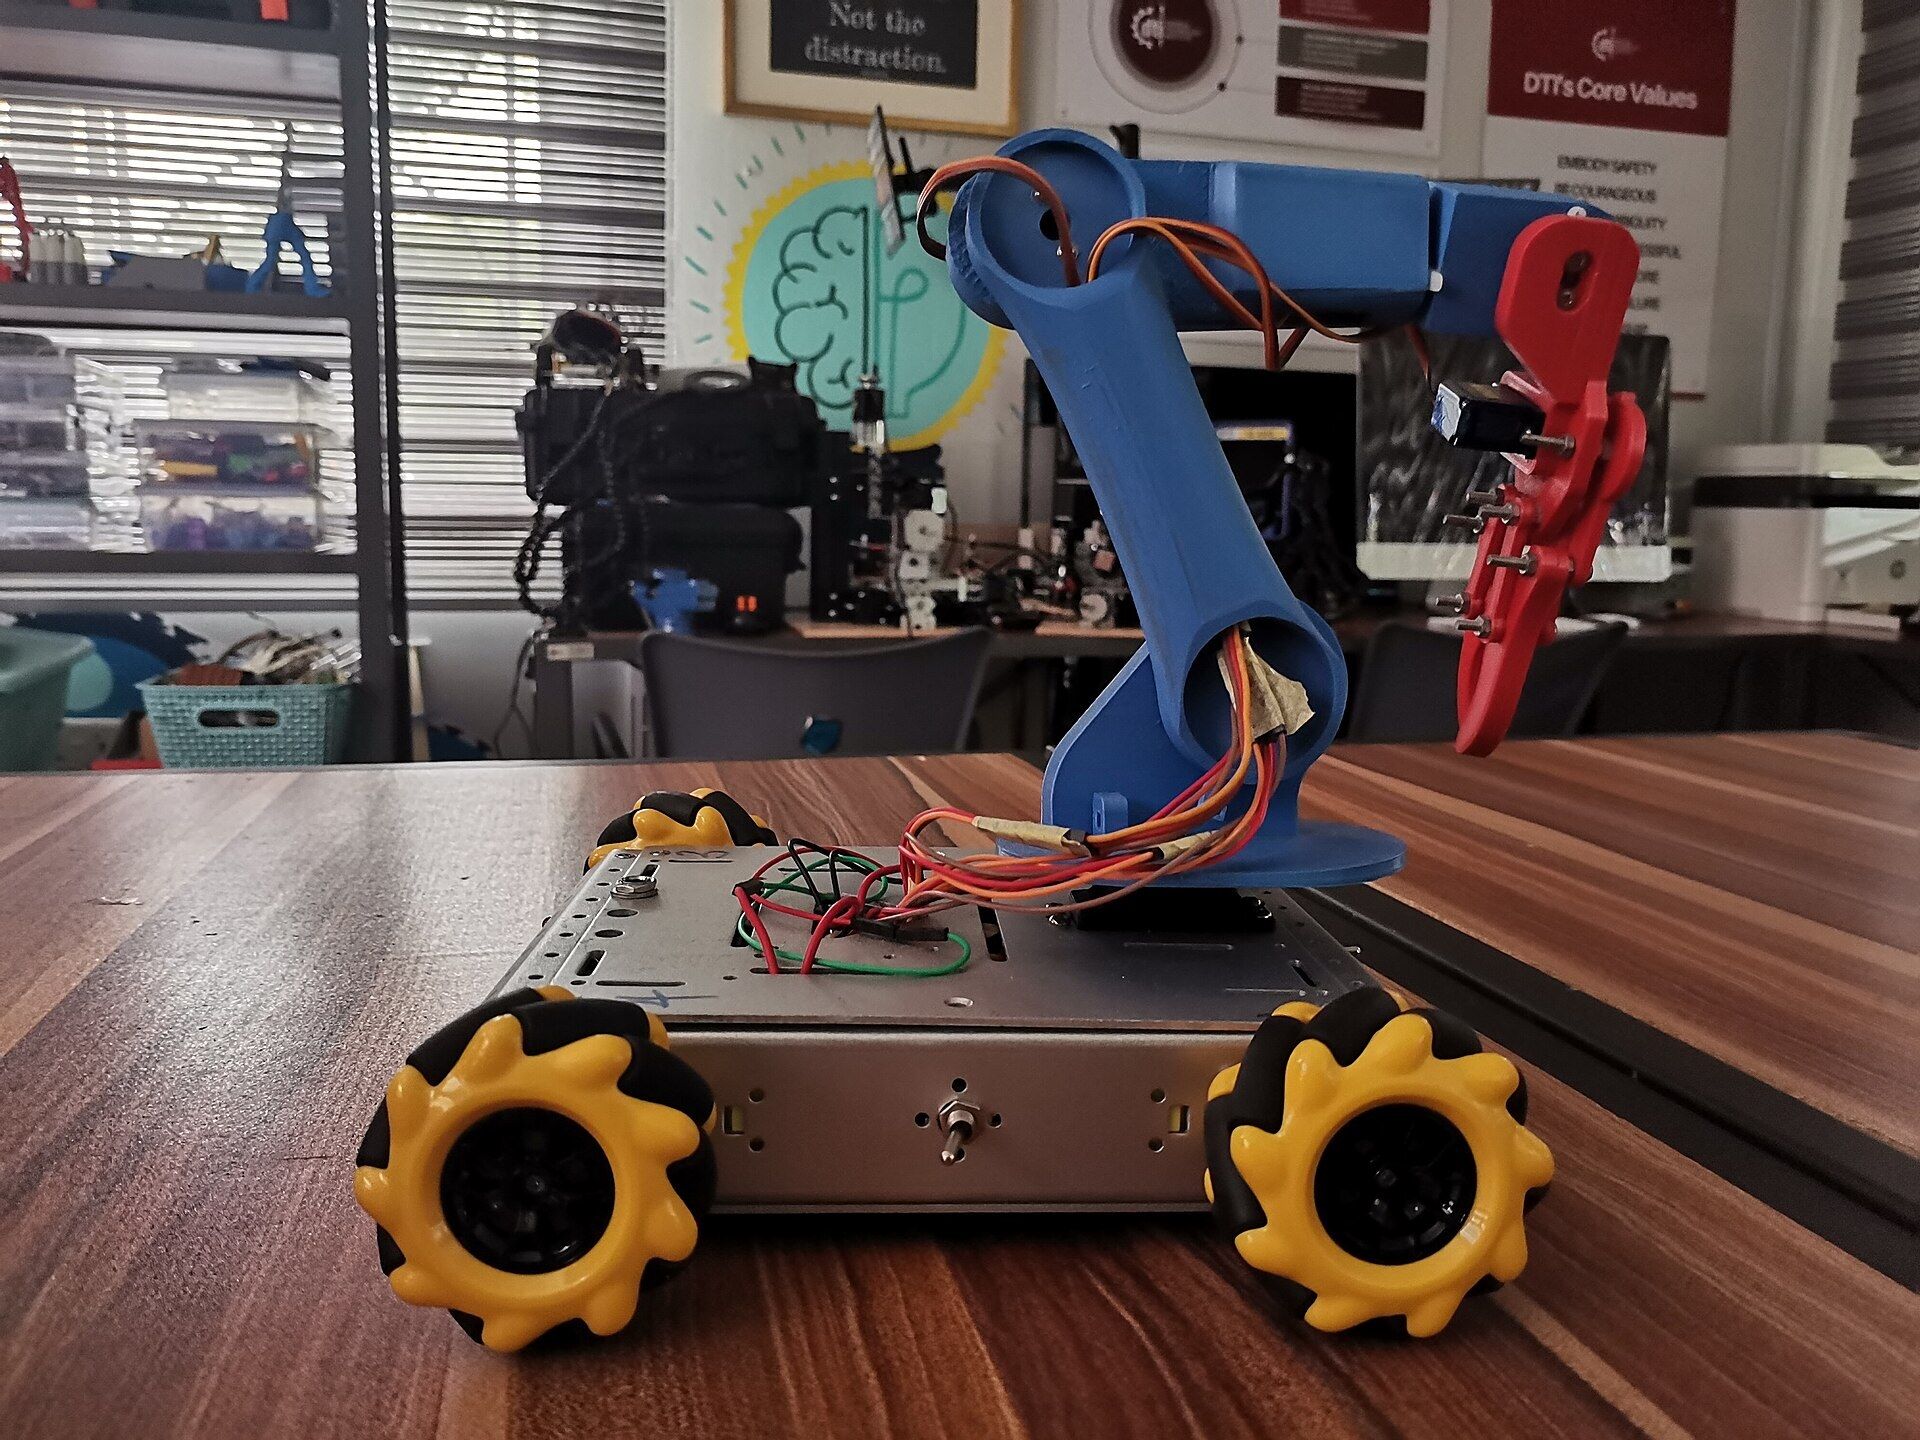
\includegraphics[width=0.80\linewidth]{image/ch05/photo-arm-mecanum.jpg}
  \caption{麦轮底盘与舵机机械臂组合成的教学机器人，即示例 A 与示例 B
  合并后的构型（照片：Anani A. George，Wikimedia Commons，CC0）}
  \label{fig:ch05-photo-arm}
\end{figure}

合计 16 行。左摇杆控制底盘，右摇杆控制机械臂；因为没有模式切换，两个
子系统每轮都会更新。注意 \texttt{RX/RY} 已经被机械臂占用，所以麦轮不能
再用右摇杆做开环自转；如果一定要自转，只能牺牲机械臂的某个轴，或者改用
两个模式并接受切换时另一子系统停止更新。

如果机械臂要加第三个舵机（例如底座偏航），可以把 P60 设为舵机，PWMA
本来就是 50\,Hz，接线和频率都够；但目标要用局部坐标，理由见上一节。
四轮 + 3 自由度大约 17--20 行动作，仍然可以放进一个模式，代价是代码更长、
每轮计算更多，建议在生成代码页看 Flash 余量和编译警告。

\subsection{排错}

常见现象、可能原因与处理见表~\ref{tab:ch05-troubleshooting}。

\begin{table}[htbp]
  \centering
  \small
  \begin{tabularx}{\linewidth}{@{}>{\raggedright\arraybackslash}p{0.28\linewidth} >{\raggedright\arraybackslash}X >{\raggedright\arraybackslash}X@{}}
    \toprule
    现象 & 可能原因 & 处理 \\
    \midrule
    输出下拉里没有 P74 & 该脚角色是“未使用”，或只选了频率没选角色 & 到“PWM 与引脚”把角色改成“平滑电机” \\
    提示“未启用底盘控制时不能保留底盘控制” & 模式里还开着保留底盘 & 关闭该开关；关闭底盘时界面通常会自动清除 \\
    表达式报“未定义变量” & 变量行排在引用行之后，或变量名拼错 & 把变量行移到前面；变量名区分大小写 \\
    表达式行没有“方向/控制方式” & 这是计算行的正常行为 & 不需要填；表达式直接写输出值 \\
    舵机不动或撞限位 & 角度超出 $\pm90^\circ$、零位错、机械卡死 & 用试算检查角度；重标零位；加 \texttt{min/max} 限幅 \\
    麦轮走斜线 & 某个轮子方向反了、辊子装反、四轮磨损不一致 & 单轮点动核对；改该行符号；检查机械 \\
    推前进却后退 & \texttt{LY} 符号与手柄标定相反 & 把 \texttt{vx} 改成 \texttt{-LY} 或 \texttt{LY} \\
    模式切换后轮子停 & 新模式没有映射这四个轮子 & 每个模式都写全四轮，或只用一个模式 \\
    摩擦轮脚不能写表达式 & 摩擦轮有专用安全栈，禁止直接写 duty & 用启停/单次/持续/摇杆油门四种方式 \\
    编译检查报环境错误 & 桌面工具链未准备好 & 先确认“生成代码”页能正常汇编；Web/Android 只做解析器校验 \\
    \bottomrule
  \end{tabularx}
  \caption{高级构型常见问题与处理}
  \label{tab:ch05-troubleshooting}
\end{table}

\section{能力边界、安全与小结}

\subsection{构型能力矩阵}

各构型与本期支持边界汇总见表~\ref{tab:ch05-capability}。

\begin{table}[htbp]
  \centering
  \small
  \begin{tabularx}{\linewidth}{@{}l l l >{\raggedright\arraybackslash}X@{}}
    \toprule
    构型 & 执行器/输出 & 典型分配 & 本期结论 \\
    \midrule
    差速四轮 & 4 电机 & P74--P77 & 内建底盘，支持 \\
    四轮麦轮 & 4 电机 & P74--P77，PWMB 10000\,Hz & 关底盘 + 表达式，支持，有示例 \\
    三轮全向 & 3 电机 & P74--P76，PWMB 10000\,Hz & 关底盘 + 表达式，支持，有示例 \\
    四轮全向 & 4 电机 & P74--P77 & 表达式可写，未给示例 \\
    舵轮四模块 & 4 电机 + 4 舵机 & P74--P77 10000\,Hz，P60/P62/P64/P66 50\,Hz & 无内建；表达式手工可拼但不推荐，无示例 \\
    2-DOF 机械臂 & 2 舵机 & MP03/MP74 & 表达式，支持，有示例 \\
    3-DOF 机械臂 & 3 舵机 & MP03/MP74 + P60 & 有条件：局部坐标、PWMA 50\,Hz \\
    四轮麦轮 + 2-DOF 臂 & 4 电机 + 2 舵机 & P74--P77 + MP03/MP74 & 支持，单模式 16 行 \\
    6-DOF/数值 IK & — & — & 不支持 \\
    \bottomrule
  \end{tabularx}
  \caption{高级构型的能力矩阵。P64/P66 可作舵机或摩擦轮；同一引脚不能同时担任两种角色，启用摩擦轮安全栈时两脚都须为摩擦轮}
  \label{tab:ch05-capability}
\end{table}

\subsection{上电与调试检查清单}

\begin{enumerate}
  \item 车架空，轮子悬空；机械臂支撑好，运动范围内没有人。
  \item 电池电压正常，保险丝/急停可用；第一次测试用低占空比（例如 3000）。
  \item 单轮点动确认转向；再确认前后、左右、斜向；最后才落地。
  \item 舵机先小角度、慢速，确认零位和方向，再逐步扩大范围。
  \item 观察电流、电调/电机/舵机温度；有异味、异响或抖动立即断电。
  \item 模式切换、上电、松手回中时，注意输出是否阶跃；表达式行没有软件
        斜坡，不能把“松手”当成“缓停”。
  \item 所有安全功能（急停、断电、机械限位）都不能只依赖软件；软件只是
        辅助。
\end{enumerate}

\subsection{本章小结}

\begin{itemize}
  \item 工程项目的“程序”就是按顺序执行的动作行；计算行只在“输入 =
        未指定”时出现，用变量和单条受限表达式描述控制律。
  \item 关闭预制底盘后，四路电机被释放；默认的 P74--P77 属于 PWMB，
        把 PWMB 设 10000\,Hz、PWMA 设 50\,Hz，就能同时带四轮和舵机。
  \item 麦轮靠 45$^\circ$ 辊子的斜向力合成平移，四轮公式是线性组合；
        全向轮靠 90$^\circ$ 辊子的切向力，三轮 120$^\circ$ 布局也能合成
        任意平移。
  \item 舵轮每个模块需要转向 + 驱动两个执行器，四模块占满 8 路；当前
        工具没有内建支持，不建议用开环舵轮直接上场。
  \item 二自由度机械臂的闭式逆解只需要 \texttt{atan2/sqrt} 和四则运算，
        可以用变量行拆开写；三自由度世界坐标目标需要 \texttt{sin/cos}，
        当前表达式白名单没有，只能用局部坐标。
  \item 所有示例都是开环的，没有编码器/陀螺仪回读；公式正确不等于实机
        安全，必须架空、限速、标定和有人值守。
\end{itemize}

\subsection*{练习}

\begin{enumerate}
  \item 把麦轮示例的除数从 2047 改成 4094，用试算算出纯前进时的最大
        duty，并解释为什么最大速度减半、换来的是什么。
  \item 把三轮全向的滚动方向改成 $\phi=90^\circ,210^\circ,330^\circ$，
        写出新的三条表达式，并说明轮子安装位置与滚动方向的关系。
  \item 把二自由度机械臂改成 $L_1=150$\,mm、$L_2=120$\,mm，重写
        \texttt{c2} 和 \texttt{q1} 里的四个常数；算出新的工作空间，并用
        试算检查两个舵机角度是否仍在 $\pm90^\circ$ 内。
\end{enumerate}
